%%%%%%%%%%%%%%%%%%%%%%%%%%%%%%%%%%%%%%%%%
% The Legrand Orange Book
% LaTeX Template
% Version 2.0 (9/2/15)
%%%%%%%%%%%%%%%%%%%%%%%%%%%%%%%%%%%%%%%%%%
%  Adaptado por Prof. Ausberto Castro Vera,
%  2013-2021
%----------------------------------------------------------------------------------------
%	PACKAGES AND OTHER DOCUMENT CONFIGURATIONS
%----------------------------------------------------------------------------------------

\documentclass[11pt,fleqn]{book} % Default font size and left-justified equations

%----------------------------------------------------------------------------------------

%%%%%%%%%%%%%%%%%%%%%%%%%%%%%%%%%%%%%%%%%
% The Legrand Orange Book
% Structural Definitions File
% Version 2.0 (9/2/15)
%
% Original author:
% Mathias Legrand (legrand.mathias@gmail.com) with modifications by:
% Vel (vel@latextemplates.com)
%
% This file has been downloaded from:
% http://www.LaTeXTemplates.com
%
% License:
% CC BY-NC-SA 3.0 (http://creativecommons.org/licenses/by-nc-sa/3.0/)
%
%%%%%%%%%%%%%%%%%%%%%%%%%%%%%%%%%%%%%%%%%% 

%----------------------------------------------------------------------------------------
%	VARIOUS REQUIRED PACKAGES AND CONFIGURATIONS
%----------------------------------------------------------------------------------------

\usepackage[top=3cm,bottom=3cm,left=3cm,right=3cm,headsep=10pt,a4paper]{geometry} % Page margins

\usepackage{graphicx} % Required for including pictures
\graphicspath{{Pictures/}} % Specifies the directory where pictures are stored

\usepackage{lipsum} % Inserts dummy text
\usepackage{here}   %
\usepackage{tikz} % Required for drawing custom shapes

\usepackage[brazil]{babel} % Brazilian Portuguese language/hyphenation

\usepackage{enumitem} % Customize lists
\setlist{nolistsep} % Reduce spacing between bullet points and numbered lists

\usepackage{booktabs} % Required for nicer horizontal rules in tables
\usepackage{indentfirst}
\usepackage{xcolor} % Required for specifying colors by name
\definecolor{ocre}{RGB}{243,102,25} % Define the orange color used for highlighting throughout the book

%----------------------------------------------------------------------------------------
%	FONTS
%----------------------------------------------------------------------------------------

\usepackage{avant} % Use the Avantgarde font for headings
%\usepackage{times} % Use the Times font for headings
\usepackage{mathptmx} % Use the Adobe Times Roman as the default text font together with math symbols from the Sym­bol, Chancery and Com­puter Modern fonts

\usepackage{microtype} % Slightly tweak font spacing for aesthetics
\usepackage[utf8]{inputenc} % Required for including letters with accents
\usepackage[T1]{fontenc} % Use 8-bit encoding that has 256 glyphs

%----------------------------------------------------------------------------------------
%	BIBLIOGRAPHY AND INDEX
%----------------------------------------------------------------------------------------
\usepackage{hyperref}

%\usepackage[style=alphabetic, citestyle=numeric, sorting=nyt, sortcites=true,
%            autopunct=true, babel=hyphen, hyperref=true, abbreviate=false,
%            backref=true, backend=biber]{biblatex}
%\addbibresource{racketbib.bib} % BibTeX bibliography file
%\defbibheading{bibempty}{}

\usepackage{calc} % For simpler calculation - used for spacing the index letter headings correctly
\usepackage{makeidx} % Required to make an index
\makeindex % Tells LaTeX to create the files required for indexing

%----------------------------------------------------------------------------------------
%	MAIN TABLE OF CONTENTS
%----------------------------------------------------------------------------------------

\usepackage{titletoc} % Required for manipulating the table of contents

\contentsmargin{0cm} % Removes the default margin

% Part text styling
\titlecontents{part}[0cm]
{\addvspace{20pt}\centering\large\bfseries}
{}
{}
{}

% Chapter text styling
\titlecontents{chapter}[1.25cm] % Indentation
{\addvspace{12pt}\large\sffamily\bfseries} % Spacing and font options for chapters
{\color{ocre!60}\contentslabel[\Large\thecontentslabel]{1.25cm}\color{ocre}} % Chapter number
{\color{ocre}}
{\color{ocre!60}\normalsize\;\titlerule*[.5pc]{.}\;\thecontentspage} % Page number

% Section text styling
\titlecontents{section}[1.25cm] % Indentation
{\addvspace{3pt}\sffamily\bfseries} % Spacing and font options for sections
{\contentslabel[\thecontentslabel]{1.25cm}} % Section number
{}
{\hfill\color{black}\thecontentspage} % Page number
[]

% Subsection text styling
\titlecontents{subsection}[1.25cm] % Indentation
{\addvspace{1pt}\sffamily\small} % Spacing and font options for subsections
{\contentslabel[\thecontentslabel]{1.25cm}} % Subsection number
{}
{\ \titlerule*[.5pc]{.}\;\thecontentspage} % Page number
[]

% List of figures
\titlecontents{figure}[0em]
{\addvspace{-5pt}\sffamily}
{\thecontentslabel\hspace*{1em}}
{}
{\ \titlerule*[.5pc]{.}\;\thecontentspage}
[]

% List of tables
\titlecontents{table}[0em]
{\addvspace{-5pt}\sffamily}
{\thecontentslabel\hspace*{1em}}
{}
{\ \titlerule*[.5pc]{.}\;\thecontentspage}
[]

%----------------------------------------------------------------------------------------
%	MINI TABLE OF CONTENTS IN PART HEADS
%----------------------------------------------------------------------------------------

% Chapter text styling
\titlecontents{lchapter}[0em] % Indenting
{\addvspace{15pt}\large\sffamily\bfseries} % Spacing and font options for chapters
{\color{ocre}\contentslabel[\Large\thecontentslabel]{1.25cm}\color{ocre}} % Chapter number
{}
{\color{ocre}\normalsize\sffamily\bfseries\;\titlerule*[.5pc]{.}\;\thecontentspage} % Page number

% Section text styling
\titlecontents{lsection}[0em] % Indenting
{\sffamily\small} % Spacing and font options for sections
{\contentslabel[\thecontentslabel]{1.25cm}} % Section number
{}
{}

% Subsection text styling
\titlecontents{lsubsection}[.5em] % Indentation
{\normalfont\footnotesize\sffamily} % Font settings
{}
{}
{}

%----------------------------------------------------------------------------------------
%	PAGE HEADERS
%----------------------------------------------------------------------------------------

\usepackage{fancyhdr} % Required for header and footer configuration

\pagestyle{fancy}
\renewcommand{\chaptermark}[1]{\markboth{\sffamily\normalsize\bfseries\chaptername\ \thechapter.\ #1}{}} % Chapter text font settings
\renewcommand{\sectionmark}[1]{\markright{\sffamily\normalsize\thesection\hspace{5pt}#1}{}} % Section text font settings
\fancyhf{} \fancyhead[LE,RO]{\sffamily\normalsize\thepage} % Font setting for the page number in the header
\fancyhead[LO]{\rightmark} % Print the nearest section name on the left side of odd pages
\fancyhead[RE]{\leftmark} % Print the current chapter name on the right side of even pages
\renewcommand{\headrulewidth}{0.5pt} % Width of the rule under the header
\addtolength{\headheight}{2.5pt} % Increase the spacing around the header slightly
\renewcommand{\footrulewidth}{0pt} % Removes the rule in the footer
\fancypagestyle{plain}{\fancyhead{}\renewcommand{\headrulewidth}{0pt}} % Style for when a plain pagestyle is specified

% Removes the header from odd empty pages at the end of chapters
\makeatletter
\renewcommand{\cleardoublepage}{
\clearpage\ifodd\c@page\else
\hbox{}
\vspace*{\fill}
\thispagestyle{empty}
\newpage
\fi}

%----------------------------------------------------------------------------------------
%	THEOREM STYLES
%----------------------------------------------------------------------------------------

\usepackage{amsmath,amsfonts,amssymb,amsthm} % For math equations, theorems, symbols, etc

\newcommand{\intoo}[2]{\mathopen{]}#1\,;#2\mathclose{[}}
\newcommand{\ud}{\mathop{\mathrm{{}d}}\mathopen{}}
\newcommand{\intff}[2]{\mathopen{[}#1\,;#2\mathclose{]}}
\newtheorem{notation}{Notation}[chapter]

% Boxed/framed environments
\newtheoremstyle{ocrenumbox}% % Theorem style name
{0pt}% Space above
{0pt}% Space below
{\normalfont}% % Body font
{}% Indent amount
{\small\bf\sffamily\color{ocre}}% % Theorem head font
{\;}% Punctuation after theorem head
{0.25em}% Space after theorem head
{\small\sffamily\color{ocre}\thmname{#1}\nobreakspace\thmnumber{\@ifnotempty{#1}{}\@upn{#2}}% Theorem text (e.g. Theorem 2.1)
\thmnote{\nobreakspace\the\thm@notefont\sffamily\bfseries\color{black}---\nobreakspace#3.}} % Optional theorem note
\renewcommand{\qedsymbol}{$\blacksquare$}% Optional qed square

\newtheoremstyle{blacknumex}% Theorem style name
{5pt}% Space above
{5pt}% Space below
{\normalfont}% Body font
{} % Indent amount
{\small\bf\sffamily}% Theorem head font
{\;}% Punctuation after theorem head
{0.25em}% Space after theorem head
{\small\sffamily{\tiny\ensuremath{\blacksquare}}\nobreakspace\thmname{#1}\nobreakspace\thmnumber{\@ifnotempty{#1}{}\@upn{#2}}% Theorem text (e.g. Theorem 2.1)
\thmnote{\nobreakspace\the\thm@notefont\sffamily\bfseries---\nobreakspace#3.}}% Optional theorem note

\newtheoremstyle{blacknumbox} % Theorem style name
{0pt}% Space above
{0pt}% Space below
{\normalfont}% Body font
{}% Indent amount
{\small\bf\sffamily}% Theorem head font
{\;}% Punctuation after theorem head
{0.25em}% Space after theorem head
{\small\sffamily\thmname{#1}\nobreakspace\thmnumber{\@ifnotempty{#1}{}\@upn{#2}}% Theorem text (e.g. Theorem 2.1)
\thmnote{\nobreakspace\the\thm@notefont\sffamily\bfseries---\nobreakspace#3.}}% Optional theorem note

% Non-boxed/non-framed environments
\newtheoremstyle{ocrenum}% % Theorem style name
{5pt}% Space above
{5pt}% Space below
{\normalfont}% % Body font
{}% Indent amount
{\small\bf\sffamily\color{ocre}}% % Theorem head font
{\;}% Punctuation after theorem head
{0.25em}% Space after theorem head
{\small\sffamily\color{ocre}\thmname{#1}\nobreakspace\thmnumber{\@ifnotempty{#1}{}\@upn{#2}}% Theorem text (e.g. Theorem 2.1)
\thmnote{\nobreakspace\the\thm@notefont\sffamily\bfseries\color{black}---\nobreakspace#3.}} % Optional theorem note
\renewcommand{\qedsymbol}{$\blacksquare$}% Optional qed square
\makeatother

% Defines the theorem text style for each type of theorem to one of the three styles above
\newcounter{dummy}
\numberwithin{dummy}{section}
\theoremstyle{ocrenumbox}
\newtheorem{theoremeT}[dummy]{Theorem}
\newtheorem{problem}{Problem}[chapter]
\newtheorem{exerciseT}{Exercise}[chapter]
\theoremstyle{blacknumex}
\newtheorem{exampleT}{Example}[chapter]
\theoremstyle{blacknumbox}
\newtheorem{vocabulary}{Vocabulary}[chapter]
\newtheorem{definitionT}{Definition}[section]
\newtheorem{corollaryT}[dummy]{Corollary}
\theoremstyle{ocrenum}
\newtheorem{proposition}[dummy]{Proposition}

%----------------------------------------------------------------------------------------
%	DEFINITION OF COLORED BOXES
%----------------------------------------------------------------------------------------

\RequirePackage[framemethod=default]{mdframed} % Required for creating the theorem, definition, exercise and corollary boxes

% Theorem box
\newmdenv[skipabove=7pt,
skipbelow=7pt,
backgroundcolor=black!5,
linecolor=ocre,
innerleftmargin=5pt,
innerrightmargin=5pt,
innertopmargin=5pt,
leftmargin=0cm,
rightmargin=0cm,
innerbottommargin=5pt]{tBox}

% Exercise box	
\newmdenv[skipabove=7pt,
skipbelow=7pt,
rightline=false,
leftline=true,
topline=false,
bottomline=false,
backgroundcolor=ocre!10,
linecolor=ocre,
innerleftmargin=5pt,
innerrightmargin=5pt,
innertopmargin=5pt,
innerbottommargin=5pt,
leftmargin=0cm,
rightmargin=0cm,
linewidth=4pt]{eBox}	

% Definition box
\newmdenv[skipabove=7pt,
skipbelow=7pt,
rightline=false,
leftline=true,
topline=false,
bottomline=false,
linecolor=ocre,
innerleftmargin=5pt,
innerrightmargin=5pt,
innertopmargin=0pt,
leftmargin=0cm,
rightmargin=0cm,
linewidth=4pt,
innerbottommargin=0pt]{dBox}	

% Corollary box
\newmdenv[skipabove=7pt,
skipbelow=7pt,
rightline=false,
leftline=true,
topline=false,
bottomline=false,
linecolor=gray,
backgroundcolor=black!5,
innerleftmargin=5pt,
innerrightmargin=5pt,
innertopmargin=5pt,
leftmargin=0cm,
rightmargin=0cm,
linewidth=4pt,
innerbottommargin=5pt]{cBox}

% Creates an environment for each type of theorem and assigns it a theorem text style from the "Theorem Styles" section above and a colored box from above
\newenvironment{theorem}{\begin{tBox}\begin{theoremeT}}{\end{theoremeT}\end{tBox}}
\newenvironment{exercise}{\begin{eBox}\begin{exerciseT}}{\hfill{\color{ocre}\tiny\ensuremath{\blacksquare}}\end{exerciseT}\end{eBox}}				
\newenvironment{definition}{\begin{dBox}\begin{definitionT}}{\end{definitionT}\end{dBox}}	
\newenvironment{example}{\begin{exampleT}}{\hfill{\tiny\ensuremath{\blacksquare}}\end{exampleT}}		
\newenvironment{corollary}{\begin{cBox}\begin{corollaryT}}{\end{corollaryT}\end{cBox}}	

%----------------------------------------------------------------------------------------
%	REMARK ENVIRONMENT
%----------------------------------------------------------------------------------------

\newenvironment{remark}{\par\vspace{10pt}\small % Vertical white space above the remark and smaller font size
\begin{list}{}{
\leftmargin=35pt % Indentation on the left
\rightmargin=25pt}\item\ignorespaces % Indentation on the right
\makebox[-2.5pt]{\begin{tikzpicture}[overlay]
\node[draw=ocre!60,line width=1pt,circle,fill=ocre!25,font=\sffamily\bfseries,inner sep=2pt,outer sep=0pt] at (-15pt,0pt){\textcolor{ocre}{R}};\end{tikzpicture}} % Orange R in a circle
\advance\baselineskip -1pt}{\end{list}\vskip5pt} % Tighter line spacing and white space after remark

%----------------------------------------------------------------------------------------
%	SECTION NUMBERING IN THE MARGIN
%----------------------------------------------------------------------------------------

\makeatletter
\renewcommand{\@seccntformat}[1]{\llap{\textcolor{ocre}{\csname the#1\endcsname}\hspace{1em}}}
\renewcommand{\section}{\@startsection{section}{1}{\z@}
{-4ex \@plus -1ex \@minus -.4ex}
{1ex \@plus.2ex }
{\normalfont\large\sffamily\bfseries}}
\renewcommand{\subsection}{\@startsection {subsection}{2}{\z@}
{-3ex \@plus -0.1ex \@minus -.4ex}
{0.5ex \@plus.2ex }
{\normalfont\sffamily\bfseries}}
\renewcommand{\subsubsection}{\@startsection {subsubsection}{3}{\z@}
{-2ex \@plus -0.1ex \@minus -.2ex}
{.2ex \@plus.2ex }
{\normalfont\small\sffamily\bfseries}}
\renewcommand\paragraph{\@startsection{paragraph}{4}{\z@}
{-2ex \@plus-.2ex \@minus .2ex}
{.1ex}
{\normalfont\small\sffamily\bfseries}}

%----------------------------------------------------------------------------------------
%	PART HEADINGS
%----------------------------------------------------------------------------------------

% numbered part in the table of contents
\newcommand{\@mypartnumtocformat}[2]{%
\setlength\fboxsep{0pt}%
\noindent\colorbox{ocre!20}{\strut\parbox[c][.7cm]{\ecart}{\color{ocre!70}\Large\sffamily\bfseries\centering#1}}\hskip\esp\colorbox{ocre!40}{\strut\parbox[c][.7cm]{\linewidth-\ecart-\esp}{\Large\sffamily\centering#2}}}%
%%%%%%%%%%%%%%%%%%%%%%%%%%%%%%%%%%
% unnumbered part in the table of contents
\newcommand{\@myparttocformat}[1]{%
\setlength\fboxsep{0pt}%
\noindent\colorbox{ocre!40}{\strut\parbox[c][.7cm]{\linewidth}{\Large\sffamily\centering#1}}}%
%%%%%%%%%%%%%%%%%%%%%%%%%%%%%%%%%%
\newlength\esp
\setlength\esp{4pt}
\newlength\ecart
\setlength\ecart{1.2cm-\esp}
\newcommand{\thepartimage}{}%
\newcommand{\partimage}[1]{\renewcommand{\thepartimage}{#1}}%
\def\@part[#1]#2{%
\ifnum \c@secnumdepth >-2\relax%
\refstepcounter{part}%
\addcontentsline{toc}{part}{\texorpdfstring{\protect\@mypartnumtocformat{\thepart}{#1}}{\partname~\thepart\ ---\ #1}}
\else%
\addcontentsline{toc}{part}{\texorpdfstring{\protect\@myparttocformat{#1}}{#1}}%
\fi%
\startcontents%
\markboth{}{}%
{\thispagestyle{empty}%
\begin{tikzpicture}[remember picture,overlay]%
\node at (current page.north west){\begin{tikzpicture}[remember picture,overlay]%	
\fill[ocre!20](0cm,0cm) rectangle (\paperwidth,-\paperheight);
\node[anchor=north] at (4cm,-3.25cm){\color{ocre!40}\fontsize{220}{100}\sffamily\bfseries\@Roman\c@part};
\node[anchor=south east] at (\paperwidth-1cm,-\paperheight+1cm){\parbox[t][][t]{8.5cm}{
\printcontents{l}{0}{\setcounter{tocdepth}{1}}%
}};
\node[anchor=north east] at (\paperwidth-1.5cm,-3.25cm){\parbox[t][][t]{15cm}{\strut\raggedleft\color{white}\fontsize{30}{30}\sffamily\bfseries#2}};
\end{tikzpicture}};
\end{tikzpicture}}%
\@endpart}
\def\@spart#1{%
\startcontents%
\phantomsection
{\thispagestyle{empty}%
\begin{tikzpicture}[remember picture,overlay]%
\node at (current page.north west){\begin{tikzpicture}[remember picture,overlay]%	
\fill[ocre!20](0cm,0cm) rectangle (\paperwidth,-\paperheight);
\node[anchor=north east] at (\paperwidth-1.5cm,-3.25cm){\parbox[t][][t]{15cm}{\strut\raggedleft\color{white}\fontsize{30}{30}\sffamily\bfseries#1}};
\end{tikzpicture}};
\end{tikzpicture}}
\addcontentsline{toc}{part}{\texorpdfstring{%
\setlength\fboxsep{0pt}%
\noindent\protect\colorbox{ocre!40}{\strut\protect\parbox[c][.7cm]{\linewidth}{\Large\sffamily\protect\centering #1\quad\mbox{}}}}{#1}}%
\@endpart}
\def\@endpart{\vfil\newpage
\if@twoside
\if@openright
\null
\thispagestyle{empty}%
\newpage
\fi
\fi
\if@tempswa
\twocolumn
\fi}

%----------------------------------------------------------------------------------------
%	CHAPTER HEADINGS
%----------------------------------------------------------------------------------------

\newcommand{\thechapterimage}{}%
\newcommand{\chapterimage}[1]{\renewcommand{\thechapterimage}{#1}}%
\def\@makechapterhead#1{%
{\parindent \z@ \raggedright \normalfont
\ifnum \c@secnumdepth >\m@ne
\if@mainmatter
\begin{tikzpicture}[remember picture,overlay]
\node at (current page.north west)
{\begin{tikzpicture}[remember picture,overlay]
\node[anchor=north west,inner sep=0pt] at (0,0) {\includegraphics[width=\paperwidth]{\thechapterimage}};
\draw[anchor=west] (\Gm@lmargin,-9cm) node [line width=2pt,rounded corners=15pt,draw=ocre,fill=white,fill opacity=0.5,inner sep=15pt]{\strut\makebox[22cm]{}};
\draw[anchor=west] (\Gm@lmargin+.3cm,-9cm) node {\huge\sffamily\bfseries\color{black}\thechapter. #1\strut};
\end{tikzpicture}};
\end{tikzpicture}
\else
\begin{tikzpicture}[remember picture,overlay]
\node at (current page.north west)
{\begin{tikzpicture}[remember picture,overlay]
\node[anchor=north west,inner sep=0pt] at (0,0) {\includegraphics[width=\paperwidth]{\thechapterimage}};
\draw[anchor=west] (\Gm@lmargin,-9cm) node [line width=2pt,rounded corners=15pt,draw=ocre,fill=white,fill opacity=0.5,inner sep=15pt]{\strut\makebox[22cm]{}};
\draw[anchor=west] (\Gm@lmargin+.3cm,-9cm) node {\huge\sffamily\bfseries\color{black}#1\strut};
\end{tikzpicture}};
\end{tikzpicture}
\fi\fi\par\vspace*{270\p@}}}

%-------------------------------------------

\def\@makeschapterhead#1{%
\begin{tikzpicture}[remember picture,overlay]
\node at (current page.north west)
{\begin{tikzpicture}[remember picture,overlay]
\node[anchor=north west,inner sep=0pt] at (0,0) {\includegraphics[width=\paperwidth]{\thechapterimage}};
\draw[anchor=west] (\Gm@lmargin,-9cm) node [line width=2pt,rounded corners=15pt,draw=ocre,fill=white,fill opacity=0.5,inner sep=15pt]{\strut\makebox[22cm]{}};
\draw[anchor=west] (\Gm@lmargin+.3cm,-9cm) node {\huge\sffamily\bfseries\color{black}#1\strut};
\end{tikzpicture}};
\end{tikzpicture}
\par\vspace*{270\p@}}
\makeatother

%----------------------------------------------------------------------------------------
%	HYPERLINKS IN THE DOCUMENTS
%----------------------------------------------------------------------------------------

\usepackage{hyperref}
\hypersetup{hidelinks,backref=true,pagebackref=true,hyperindex=true,colorlinks=false,breaklinks=true,urlcolor= ocre,bookmarks=true,bookmarksopen=false,pdftitle={Title},pdfauthor={Author}}
\usepackage{bookmark}
\bookmarksetup{
open,
numbered,
addtohook={%
\ifnum\bookmarkget{level}=0 % chapter
\bookmarksetup{bold}%
\fi
\ifnum\bookmarkget{level}=-1 % part
\bookmarksetup{color=ocre,bold}%
\fi
}
}

\usepackage[many]{tcolorbox}
\tcbset{skin=enhanced}



%----------------------------------------------------------------------------------------
%	Listings CSS JavaScript
%----------------------------------------------------------------------------------------
\usepackage{listings}
\definecolor{light-gray}{gray}{0.40}

% CSS
\lstdefinelanguage{CSS}{
  keywords={color,background-image:,margin,padding,font,weight,display,position,top,left,right,bottom,list,style,border,size,white,space,min,width, transition:, transform:, transition-property, transition-duration, transition-timing-function},	
  sensitive=true,
  morecomment=[l]{//},
  morecomment=[s]{/*}{*/},
  morestring=[b]',
  morestring=[b]",
  alsoletter={:},
  alsodigit={-}
}

% JavaScript
\lstdefinelanguage{JavaScript}{
  morekeywords=[1]{typeof, new, true, false, catch, function, return, null, catch, switch, var, if, in, while, do, else},
  morekeywords=[2]{case, break, input, print, char },
  morecomment=[s]{/*}{*/},
  morecomment=[l]//,
  morestring=[b]",
  morestring=[b]'
  moredelim=**[is][\color{light-gray}]{<<@<<}{>>@>>},
  moredelim=**[is][\itshape\color{OliveGreen}]{<<;<<}{>>;>>},
  morecomment=[s]{\#|}{|\#},
  sensitive=true,
%  basicstyle=\small\ttfamily,
%  keywordstyle=\bf\ttfamily\color[rgb]{0,.3,.7},
  commentstyle=\color[rgb]{0.133,0.545,0.133},
  stringstyle={\color[rgb]{0.75,0.49,0.07}},
}

\definecolor{mygreen}{rgb}{0,0.6,0}
\definecolor{mygray}{rgb}{0.5,0.5,0.5}
\definecolor{mymauve}{rgb}{0.58,0,0.82}
\lstset{
  language=JavaScript,                 % the language of the code
  backgroundcolor=\color{white},   % choose the background color; you must add \usepackage{color} or
                                   % \usepackage{xcolor}; should come as last argument
  basicstyle=\footnotesize,        % the size of the fonts that are used for the code
  breakatwhitespace=false,         % sets if automatic breaks should only happen at whitespace
  breaklines=true,                 % sets automatic line breaking
  captionpos=b,                    % sets the caption-position to bottom
  commentstyle=\color{mygreen},    % comment style
  deletekeywords={...},            % if you want to delete keywords from the given language
  escapeinside={\%*}{*)},          % if you want to add LaTeX within your code
  extendedchars=true,              % lets you use non-ASCII characters; for 8-bits encodings only, does not work with UTF-8
  %firstnumber=10,                  % start line enumeration with line 10
  %frame=single,	                   % adds a frame around the code
  keepspaces=true,                 % keeps spaces in text, useful for keeping indentation of code (possibly needs columns=flexible)
  keywordstyle=\color{blue},       % keyword style
  morekeywords={*,...},            % if you want to add more keywords to the set
  numbers=left,                    % where to put the line-numbers; possible values are (none, left, right)
  numbersep=5pt,                   % how far the line-numbers are from the code
  numberstyle=\tiny\color{mygray}, % the style that is used for the line-numbers
  rulecolor=\color{black},         % if not set, the frame-color may be changed on line-breaks within not-black text (e.g. comments (green here))
  showspaces=false,                % show spaces everywhere adding particular underscores; it overrides 'showstringspaces'
  showstringspaces=false,          % underline spaces within strings only
  showtabs=false,                  % show tabs within strings adding particular underscores
  stepnumber=2,                    % the step between two line-numbers. If it's 1, each line will be numbered
  stringstyle=\color{mymauve},     % string literal style
  tabsize=2,	                   % sets default tabsize to 2 spaces
  title=\lstname                   % show the filename of files included with \lstinputlisting; also try caption instead of title
}







\lstdefinelanguage{HTML5}{
  language=html,
  sensitive=true,	
  alsoletter={<>=-},	
  morecomment=[s]{<!-}{-->},
  tag=[s],
  otherkeywords={
  % General
  >,
  % Standard tags
	<!DOCTYPE,
  </html, <html, <head, <title, </title, <style, </style, <link, </head, <meta, />,
	% body
	</body, <body,
	% Divs
	</div, <div, </div>,
	% Paragraphs
	</p, <p, </p>,
	% scripts
	</script, <script,
  % More tags...
  <canvas, /canvas>, <svg, <rect, <animateTransform, </rect>, </svg>, <video, <source, <iframe, </iframe>, </video>, <image, </image>, <header, </header, <article, </article
  },
  ndkeywords={
  % General
  =,
  % HTML attributes
  charset=, src=, id=, width=, height=, style=, type=, rel=, href=,
  % SVG attributes
  fill=, attributeName=, begin=, dur=, from=, to=, poster=, controls=, x=, y=, repeatCount=, xlink:href=,
  % properties
  margin:, padding:, background-image:, border:, top:, left:, position:, width:, height:, margin-top:, margin-bottom:, font-size:, line-height:,
	% CSS3 properties
  transform:, -moz-transform:, -webkit-transform:,
  animation:, -webkit-animation:,
  transition:,  transition-duration:, transition-property:, transition-timing-function:,
  }
  moredelim=**[is][\color{light-gray}]{<<@<<}{>>@>>},
  moredelim=**[is][\itshape\color{OliveGreen}]{<<;<<}{>>;>>},
  morecomment=[s]{\#|}{|\#},
  sensitive=true,
  basicstyle=\small\ttfamily,
  keywordstyle=\bf\ttfamily\color[rgb]{0,.3,.7},
  commentstyle=\color[rgb]{0.133,0.545,0.133},
  stringstyle={\color[rgb]{0.75,0.49,0.07}},
}

\lstdefinestyle{htmlcssjs} {%
  % General design
%  backgroundcolor=\color{editorGray},
  basicstyle={\footnotesize\ttfamily},
  frame=b,
  % line-numbers
  xleftmargin={0.75cm},
  numbers=left,
  stepnumber=1,
  firstnumber=1,
  numberfirstline=true,	
  % Code design
  identifierstyle=\color{black},
  keywordstyle=\color{blue}\bfseries,
  ndkeywordstyle=\color{editorGreen}\bfseries,
  stringstyle=\color{editorOcher}\ttfamily,
  commentstyle=\color{brown}\ttfamily,
  % Code
  language=HTML5,
  alsolanguage=JavaScript,
  alsodigit={.:;},	
  tabsize=2,
  showtabs=false,
  showspaces=false,
  showstringspaces=false,
  extendedchars=true,
  breaklines=true,
  % German umlauts
  literate=%
  {\"{O}}{\"{O}}1
  {\"{A}}{\"{A}}1
  {\"{U}}{\"{U}}1
  {{\ss}}{{\ss}}1
  {\"{u}}{\"{u}}1
  {\"{a}}{\"{a}}1
  {\"{o}}{\"{o}}1
}
%


%----------------------------------------------------------------------------------------
%	
%----------------------------------------------------------------------------------------

\usepackage[brazilian,hyperpageref]{backref}
% Configura\c{c}\~{o}es do pacote backref
% Usado sem a op\c{c}\~{a}o hyperpageref de backref
\renewcommand{\backrefpagesname}{Citado na(s) p\'{a}gina(s):~}
% Texto padr\~{a}o antes do n\'{u}mero das p\'{a}ginas
\renewcommand{\backref}{}
% Define os textos da cita\c{c}\~{a}o
\renewcommand*{\backrefalt}[4]{
	\ifcase #1 %
		Nenhuma cita\c{c}\~{a}o no texto.%
	\or
		Citado na p\'{a}gina #2.%
	\else
		Citado #1 vezes nas p\'{a}ginas #2.%
	\fi}%
% ---


\sloppy


\hypersetup{
    bookmarks=true,         % show bookmarks bar?
    unicode=false,          % non-Latin characters in Acrobat’s bookmarks
    pdftoolbar=true,        % show Acrobat’s toolbar?
    pdfmenubar=true,        % show Acrobat’s menu?
    pdffitwindow=true,     % window fit to page when opened
    pdfstartview={FitH},    % fits the width of the page to the window
    pdftitle={Tutorial sobre a Linguagem Racket},    % title
  %  pdfauthor={Mariana A. Gualhano and Ausberto S. Castro Vera},     % author
    pdfsubject={Paradigmas de Linguagens de Programa\c{c}\~{a}o},   % subject of the document
    pdfcreator={ASCV, WinEdt},   % creator of the document
    pdfproducer={ASCV}, % producer of the document
    pdfkeywords={Programa\c{c}\~{a}o} {Funcional} {Paradigmas}, % list of keywords
    pdfnewwindow=true,      % links in new window
    colorlinks=true,       % false: boxed links; true: colored links
    linkcolor=ocre,          % color of internal links (change box color with linkbordercolor)
    citecolor=blue,        % color of links to bibliography
    filecolor=magenta,      % color of file links
    urlcolor=cyan           % color of external links
}	
 % Insert the commands.tex file which contains the majority of the structure behind the template
%Define the listing package
\usepackage{listings} %code highlighter
\usepackage{color} %use color
\definecolor{mygreen}{rgb}{0,0.6,0}
\definecolor{mygray}{rgb}{0.5,0.5,0.5}
\definecolor{mymauve}{rgb}{0.58,0,0.82}

%Customize a bit the look
\lstset{ %
	backgroundcolor=\color{white}, % choose the background color; you must add \usepackage{color} or \usepackage{xcolor}
	basicstyle=\footnotesize, % the size of the fonts that are used for the code
	breakatwhitespace=false, % sets if automatic breaks should only happen at whitespace
	breaklines=true, % sets automatic line breaking
	captionpos=b, % sets the caption-position to bottom
	commentstyle=\color{mygreen}, % comment style
	deletekeywords={...}, % if you want to delete keywords from the given language
	escapeinside={\%*}{*)}, % if you want to add LaTeX within your code
	extendedchars=true, % lets you use non-ASCII characters; for 8-bits encodings only, does not work with UTF-8
	frame=single, % adds a frame around the code
	keepspaces=true, % keeps spaces in text, useful for keeping indentation of code (possibly needs columns=flexible)
	keywordstyle=\color{blue}, % keyword style
	% language=Octave, % the language of the code
	morekeywords={*,...}, % if you want to add more keywords to the set
	numbers=left, % where to put the line-numbers; possible values are (none, left, right)
	numbersep=5pt, % how far the line-numbers are from the code
	numberstyle=\tiny\color{mygray}, % the style that is used for the line-numbers
	rulecolor=\color{black}, % if not set, the frame-color may be changed on line-breaks within not-black text (e.g. comments (green here))
	showspaces=false, % show spaces everywhere adding particular underscores; it overrides 'showstringspaces'
	showstringspaces=false, % underline spaces within strings only
	showtabs=false, % show tabs within strings adding particular underscores
	stepnumber=1, % the step between two line-numbers. If it's 1, each line will be numbered
	stringstyle=\color{mymauve}, % string literal style
	tabsize=2, % sets default tabsize to 2 spaces
	title=\lstname % show the filename of files included with \lstinputlisting; also try caption instead of title
}
%END of listing package%

\definecolor{darkgray}{rgb}{.4,.4,.4}
\definecolor{purple}{rgb}{0.65, 0.12, 0.82}

%define Javascript language
\lstdefinelanguage{JavaScript}{
	keywords={typeof, new, true, false, catch, function, return, null, catch, switch, var, if, in, while, do, else, case, break},
	keywordstyle=\color{blue}\bfseries,
	ndkeywords={class, export, boolean, throw, implements, import, this},
	ndkeywordstyle=\color{darkgray}\bfseries,
	identifierstyle=\color{black},
	sensitive=false,
	comment=[l]{//},
	morecomment=[s]{/*}{*/},
	commentstyle=\color{purple}\ttfamily,
	stringstyle=\color{red}\ttfamily,
	morestring=[b]',
	morestring=[b]"
}

\lstset{
	language=JavaScript,
	extendedchars=true,
	basicstyle=\footnotesize\ttfamily,
	showstringspaces=false,
	showspaces=false,
	numbers=left,
	numberstyle=\footnotesize,
	numbersep=9pt,
	tabsize=2,
	breaklines=true,
	showtabs=false,
	captionpos=b
}

\begin{document}

%----------------------------------------------------------------------------------------
%	TITLE PAGE
%----------------------------------------------------------------------------------------

\begingroup
\thispagestyle{empty}
\begin{tikzpicture}[remember picture,overlay]
\coordinate [below=12cm] (midpoint) at (current page.north);
\node at (current page.north west)
{\begin{tikzpicture}[remember picture,overlay]
\node[anchor=north west,inner sep=0pt] at (0,0)
        {
\includegraphics[width=\paperwidth]{capa}}; %Capa Imagem A4 21x29.7
\draw[anchor=north] (midpoint) node [fill=ocre!30!white,fill opacity=0.6,text opacity=1,inner sep=1cm]{\Huge\centering\bfseries\sffamily\parbox[c][][t]
        {\paperwidth}
        {\centering Introdu\c{c}\~{a}o \`{a} Linguagem JavaScript\\[5pt] % Titulo Livro
{\Large Paradigmas de Linguagens de Programa\c{c}\~{a}o}\\[20pt] % Subtitle
{\huge \color{blue} Gabriel Marques de Amaral Gravina}\\ % Autor nome
{\huge  \color{blue} Ausberto S. Castro Vera}\\
{\small \today}
}}; % Autor nome
\end{tikzpicture}};
\end{tikzpicture}
\vfill

\endgroup

%----------------------------------------------------------------------------------------
%	COPYRIGHT PAGE
%----------------------------------------------------------------------------------------

\newpage
~\vfill
\thispagestyle{empty}

\noindent Copyright \copyright\  \the\year{} Gabriel Marques de Amaral Gravina e Ausberto S. Castro Vera\\ % Copyright notice

\noindent \textsc{UENF - Universidade Estadual do Norte Fluminense Darcy Ribeiro}\\ % Universidade

\noindent \textsc{CCT - Centro de Ci\^{e}ncia e Tecnologia}\\ % Centro
\noindent \textsc{LCMAT - Laborat\'{o}rio de Matem\'{a}ticas}\\ % Laboratorio
\noindent \textsc{CC - Curso de Ci\^{e}ncia da Computa\c{c}\~{a}o}\\ % Curso

%\input{autor.tex} \\

\noindent \textit{Primeira edi\c{c}\~{a}o, Maio 2019} % Printing/edition date

%----------------------------------------------------------------------------------------
%	TABLE OF CONTENTS
%----------------------------------------------------------------------------------------

\chapterimage{sumariojs} % Table of contents heading image

\pagestyle{empty} % No headers

\addtocontents{toc}{\protect{\pdfbookmark[0]{\contentsname}{toc}}}
\tableofcontents % Print the table of contents itself

\cleardoublepage % Forces the first chapter to start on an odd page so it's on the right

\pagestyle{fancy} % Print headers again

%----------------------------------------------------------------------------------------
%	PART
%----------------------------------------------------------------------------------------
%\part{Part One}

%----------------------------------------------------------------------------------------
%	CHAPTERS
%----------------------------------------------------------------------------------------
\chapterimage{capitulo01.jpg} % Chapter heading image
% Prof. Dr. Ausberto S. Castro Vera
% UENF - CCT - LCMAT - Curso de Ci\^{e}ncia da Computa\c{c}\~{a}o
% Campos, RJ,  2021
% Disciplina: Paradigmas de Linguagens de Programa\c{c}\~{a}o




\chapter{ Introdu\c{c}\~{a}o}

A linguagem de programação JavaScript é a “linguagem da web”. Seu uso é dominante na internet e praticamente quase todos os sites a utilizam. 
Além disso, smartphones, tablets e vários outros dispositivos têm interpretadores de JavaScript embutidos. 
Isso a torna uma das linguagens mais utilizadas dos dias atuais e uma das linguagens mais usadas por desenvolvedores de software. 
É importante dizer que, embora o nome sugira, JavaScript é uma linguagem completamente diferente e independente da linguagem Java. 
Mesmo assim, suas sintaxes tem traços de semelhança, mas nada além disso. \newline

Por ser uma linguagem fácil de ser aprendida e fortemente tolerante, permitiu que usuários pudessem ter suas necessidades 
atendidas de forma cômoda e eficiente.
 A linguagem é de alto-nível, dinâmica e interpretada. Além disso, é adequada para orientação a objeto e programação funcional. 
 É uma linguagem não tipada – ou seja, suas variáveis não tem um tipo específico e seus tipos não são importantes para a linguagem. 
Baseado no livro \cite{flanagan2020javascript}.

\section{Aspectos hist\'{o}ricos da linguagem JavaScript}
   
A linguagem foi criada na NETSCAPE por Brendan Eich. Tecnicamente, JavaScript é uma marca registrada da Sun Microsystems (atualmente Oracle) usada para descrever a implementação da língua pela Netscape (atualmente Mozilla). Na época, a Netscape enviou a linguagem para a padronização da ECMA – European Computer Manufacturer’s Association, e sua versão padronizada ficou conhecida como “ECMAScript”. Na prática, todos chamam a linguagem apenas de JavaScript.
De acordo com \cite{flanagan2020javascript}.



   \section{\'{A}reas de Aplica\c{c}\~{a}o da Linguagem}

   A linguagem JavaScript é completamente versátil e tem aplicações nos mais variados ambientes, seja no client-side ou no server-side. 
   Nesta seção
   falarei de algumas aplicações e paradigmas da programação que podem ser implementados em JavaScript.

        \subsection{NodeJS}
        A linguagem foi criada para ser utilizada em navegadores da web, e esse segue sendo seu ambiente mais comum de execução até hoje. Enfim, o ambiente do navegador permite a linguagem obter a entrada de usuários e fazer requests HTTP. Porém, em 2010 outro ambiente foi criado para executar código em JavaScript. 
O NodeJS, popularmente conhecido como Node, tinha a ideia de invés de manter a linguagem presa a um navegador, 
permitir que a linguagem tivesse acesso ao sistema operacional. Isso proporcionou a utilização da linguagem no lado do servidor, invés de se limitar apenas ao navegador. Atualmente, o Node tem grande popularidade na implementação de servidores web.
Baseado no livro \cite{flanagan2020javascript}.
        \subsection{ Orienta\c{c}\~{a}o a objetos}
        A linguagem é orientada a objeto, porém apresenta algumas diferenças que valem ser mencionadas. 
        Na linguagem, as classes são baseadas no mecanismo de herança de protótipos. Se dois objetos herdam do mesmo objeto protótipo, então diz-se que são instâncias de uma mesma classe. 
        Membros, ou instâncias da classe, tem suas propriedades para manter e também métodos que definem seu comportamento. Este comportamento é definido pela classe e compartilhado para todas as instancias.
Retirado do artigo da documentação da linguagem, em: \url{https://developer.mozilla.org/en-US/docs/Web/JavaScript/Reference/Classes}
         \subsection{Programação Funcional}
         Basicamente, a programação funcional é um paradigma da programação que visa produzir software através de funções puras, 
         evitando compartilhamento de estados, dados mutáveis e efeitos colaterais.
         Embora JavaScript não seja uma lingugagem de programação funcional como Haskel ou Lisp, 
         o fato da linguagem poder manipular funções como objeto significa que técnicas de programação funcional podem ser implementadas na linguagem.
         Os metodos de array do ECMAScript 5, como map() e reduce() satisfazem bem o estilo de programação funcional. 
         Retirado do livro \cite{powers2015javascript}.
       

\chapterimage{capitulo.jpg} % Chapter heading image
% Prof. Dr. Ausberto S. Castro Vera
% UENF - CCT - LCMAT - Curso de Ci\^{e}ncia da Computa\c{c}\~{a}o
% Campos, RJ,  2021
% Disciplina: Paradigmas de Linguagens de Programa\c{c}\~{a}o



\chapter{ Conceitos b\'{a}sicos da Linguagem JavaScript}

Neste cap\'{\i}tulo \'{e} serão apresentados os principais conceitos da linguagem JavaScript, sua estrutura léxica, operadores, laços de repetição entre outros tópicos.
Os livros b\'{a}sicos e recomendados o estudo da Linguagem JavaScript s\~{a}o: \cite{flanagan2020javascript}, \cite{powers2015javascript} entre outros.


\section{Estrutura Léxica}
A linguagem JavaScript é feita utilizando o set de caracteres Unicode, que dá suporte a praticamente todas as linguagens utilizadas
atualmente no mundo. Essa é uma linguagem case sensitive, ou seja, os nomes de variáveis, funções e outros identificadores devem ser sempre utilizados de maneira consistente, ao contrário do que acontece no html, por exemplo. %Necessário melhorar +/-
Além disso, o JavaScript ignora os espaços e as quebras de linha, com algumas exceções. Isso permite que os programas sejam identados de maneira que façam o código ser legível e fácil de entender.
Falando em tornar o código legível, os comentários em JavaScript podem ser feitos de duas formas: uma delas são os comentários de uma só linha, que utilizam "//" e a outra são os comentários de múltiplas linhas, que ignorarão tudo que está dentro dos caracteres.
Observe o exemplo abaixo:
\newline
\begin{lstlisting}[language=JavaScript]
/*  Explicacao do codigo
	O codigo abaixo realiza... */
var helloWorld = function(){
	console.log('Hello World!');
}
helloWorld();
\end{lstlisting}
*No JavaScript o uso de vírgulas é opcional.
 


   \begin{figure}[H]
    \begin{center}
        \caption{Melhores Livros} \label{livros}
        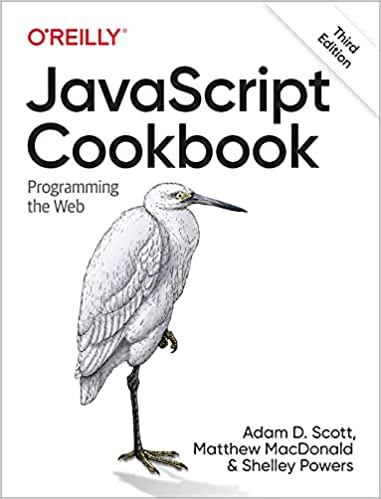
\includegraphics[width=6cm]{2021} 
                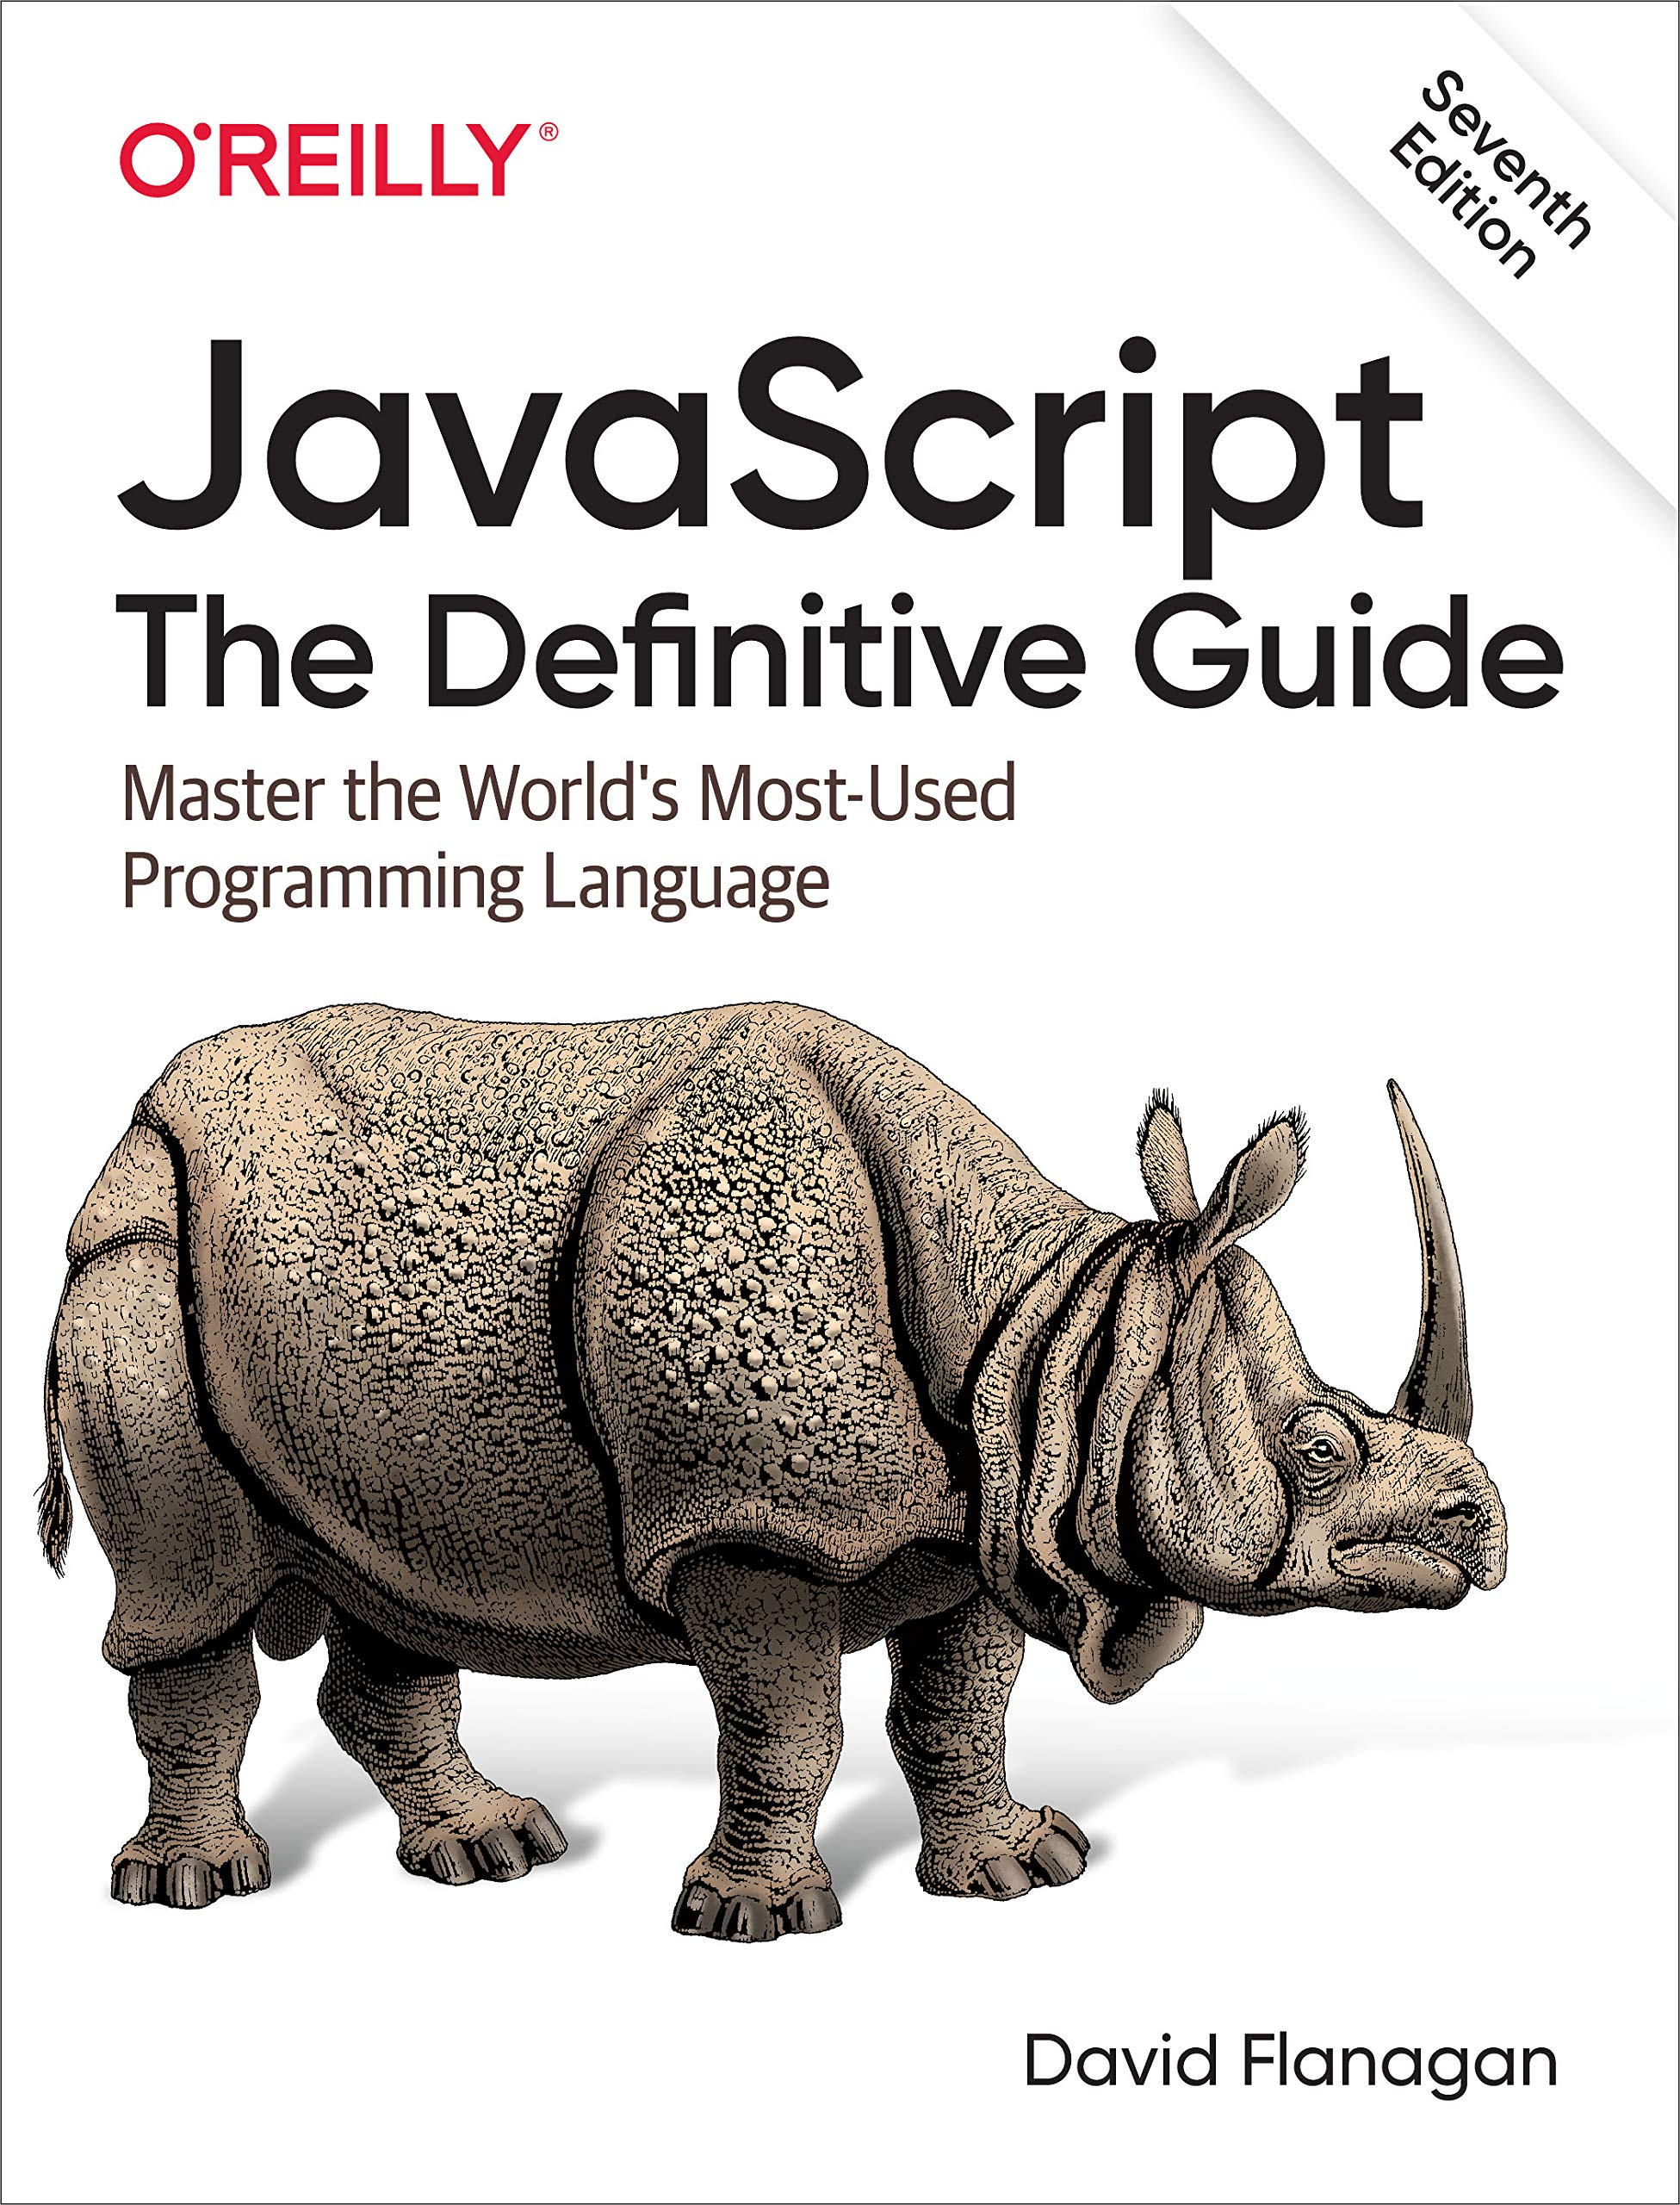
\includegraphics[width=6cm]{2020b}
        {\tiny \sf Fonte: O autor }
    \end{center}
   \end{figure} 
    %%%%%%%%=================================
    \section{Operadores}
    \begin{lstlisting}
    ++								//incremento
    --								//decremento
    !								//inverte valores em booleano
    ==								//testa equalidade
    !=								//testa inequalidade
    //testa por equalidade estrita, ou seja, o tipo tambem tem que ser o mesmo
    ===	
    ||								//OR
    &&								//AND
    =								//Atribui um valor a uma variavel
    *=, /=, %=, +=...				//Faz uma atribuicao e um calculo
    //Menor que, maior que, menor ou igual que, maior ou igual que
    <, >, <=, >=
    \end{lstlisting}
    \section{Vari\'{a}veis e Constantes}
    %%%%%%%%=================================
    Com base no livro\cite{flanagan2020javascript}, uma variável é, de forma resumida, um nome simbólico para um valor armazenado no computador. Quando chamamos uma variável, estamos acessando o valor guardado por ela. 
   	\par Na linguagem JavaScript, existem dois tipos de variáveis: as primitivas e as de objeto. 
    Para se declarar uma no JavaScript é necessário utilizar a palavra reservada "var" seguida de seu nome. Abaixo encontram-se exemplos da declaração de variáveis no JavaScript:
    \newline
    
    \begin{lstlisting}
    //E possivel declarar uma variavel vazia
    var a;
    var b = 100;
    var name = "Lucas";
    
    //Tambem e possivel declarar multiplas variaveis numa so linha
    var A = 0, B = 1, C = 2;
    
    //Variaveis tambem podem ser criadas dentro de lacos de repeticao
    (for var i = 0; i<10; i++){
    	console.log(i)
    }
    \end{lstlisting}
    
    \subsection{Tipos Primitivos}
    
	Os tipos primitivos do JS incluem números, strings de textos e valores booleanos (true e false).
	Além disso, existem também os tipos especiais "null" e "undefined", que são valores primitivos, porém não são números, strings ou booleanos. Nesse sentido, cada um é considerado membro de um tipo especial.  
	\subsubsection{Números}
	%TALVEZ Desconsiderar essa subsection
	Uma fator da linguagem JavaScript que é incomum em outras línguas é que \part{title}não há distinção entre inteiros e floats, sendo todos os números representados como floats. 
	A linguagem armazena os números utilizando o formato de floats de 64 bits, podendo armazenar números grandes com precisão considerável.
	
	\subsubsection{Strings}
	De acordo com \cite{flanagan2020javascript}, uma string é uma sequência imutável de valores de 16 bits, onde cada um representa geralmente um caractere Unicode. O tamanho da string dependerá de quantos desses valores ela contém. Para incluir uma string num programa, basta colocar aspas (simples ou duplas). Por exemplo:
	\newline
	
	\begin{lstlisting}
	//E uma string vazia
	''
	
	"10.24"	
	//Utilizacao da combinacao de aspas simples e duplas
	'O numero "8" e par'				
	
	mensagemOla = "Ola, seja bem vindo" 
	//Printa o conteudo da variavel no console do navegador
	console.log(mensagemOla)	
	
	/*compara o valor da variavel e retorna true ou false. 
	No caso, retornara true*/
	a = "Ola"
	a == "Ola"
	
	
	\end{lstlisting}
	
	\subsubsection{Booleanos}
	Conforme \cite{powers2015javascript}, um valor booleano é um valor que representa verdade ou falsidade. Deste modo, só há dois possíveis valores para um booleano. No JavaScript, as palavras reservadas para os booleanos são "true" e "false", e são geralmente o resultado de uma comparação. Observe o exemplo:
	\newline
	
	\begin{lstlisting}
		a = 10
		b = 3
		a == b
		false
		
		a == 10
		true
	\end{lstlisting}
	\subsubsection{Tipos Especiais}
	Consoante a \cite{flanagan2020javascript}, "null" é uma palavra reservada que geralmente indica ausência de um valor. Se utilizarmos o comando "typeof" no "null", veremos que será retornado "object", o que significa que "null" é algo que indica a ausência de objeto. Resumindo, pode ser utilizado para indicar que não há valor em uma variável, string ou objeto. 
	
	Por isso, "null" e "undefined" costumam ser definidos como um único objeto do seu tipo.
	
	
	\subsection{Tipos de Objeto}
	Segundo \cite{flanagan2020javascript}, qualquer valor que não seja um número, string, objeto ou null e undefined é um objeto, ou seja, é uma coleção de propriedades onde cada uma tem um nome e valor.
	
	\subsubsection{Globais}
	Os objetos globais são aqueles que podem ser usados em todo programa escrito em JavaScript. Quando um interpretador da linguagem inicia, ele cria novos objetos globais e os dá as propriedades que o definem. 
	Algumas das propriedades globais existente são: undefined, Infinity, NaN.
	Além de propriedades e funções globais, no JavaScript existem também constructor functions, como: Date(), Object() e objetos globais, como o Math e JSON.
	
	São exemplos de funções globais: 
	\newline
	\begin{lstlisting}
	isNan()			  	//Retorna se um valor e um numero ou nao.
	parseInt()		  //Recebe o conteudo de uma string e converte para. inteiro
	parseFloat() 	  //Recebe uma string e a converte para float.
	eval()	  		  //Avalia codigo representado por uma string.
	isFinite()		  //Verifica se um numero e finito.
	
	\end{lstlisting}
	
	
	\section{Estrutura de Controle e Funções}
	De acordo com \cite{flanagan2020javascript}, uma estrutura de controle dita a ordem em que instruções serão execudas. Estruturas muito conhecidas em outras linguagens estão presentes também no JavaScript.
	
	\subsection{O comando IF}
	O comando IF funciona para fazer com que o JavaScript execute expressões condicionalmente. Isso significa que o computador somente executará uma determinada instrução caso a condição seja verdadeira. Caso a seja falsa, o programa executará outro do bloco de código.
	O comando IF na linguagem toma a seguinte forma:
	\newline
	
	\begin{lstlisting}
		//Sintaxe
		if(condicao){
			//realiza instrucao A
		}else{
			//realiza outra instrucao
		}
		
		//-----Exemplo-----
		var nome = "Marcos"
		
		if(nome == Marcos){
			console.log("Bem vindo, Marcos!")
		}else{
			console.log("Apenas Marcos pode ler esta mensagem!")
		}
	\end{lstlisting}
	
	É possível também utilizar IFs dentro de outros IFs, como no exemplo abaixo:
	\newline
	\begin{lstlisting}
	
		if(animal == cachorro){
			console.log("Um cachorro e um animal")
			if(cachorro == panda){
				console.log("Um panda e um cachorro)
			}else{
				console.log("Um panda nao e um cachorro")
			}
		}
		
	\end{lstlisting}
	
	\subsection{Laços de Repetição}
	Laços de repetição executam uma instrução até que uma determinada condição seja verdadeira. Na linguagem JavaScript, os laços de repetição são o 'while', 'do ... while' e o 'for'.
	\newline
	\newline
	
	\subsubsection{While}
	Os laços de repetição "while" tem a seguinte sintaxe no JavaScript:
	\newline
	\begin{lstlisting}
		while(condicao == true){
			execute...
		}
		
		//O progrma abaixo conta de 0 a 999
		vai i = 0;
		
		while(i < 1000){
			console.log(i)
			i++
		}
		
	\end{lstlisting}
	É importante que o laço "while" atinga em algum momento uma condição de saída. Caso contrário, o programa continuará executando indefinidamente. No exemplo abaixo, temos um programa sem condição de saída.
	\newline
	\begin{lstlisting}
		while(Bolsonaro == Horroroso){
			console.log("O presidente e horroroso")
		}
		//O programa printara a mensagem acima indefinidamente
	\end{lstlisting}
	
	\subsection{For}
	
	Geralmente, os laços que utilizam o "for" são mais simples de serem lido. Isso devido ao fato de poderem executar uma variável inicial, testá-la e incrementála em uma única linha. Na linguagem, o laço for funciona com a seguinte sintaxe:
	\newline
	\begin{lstlisting}
		for(inicia variavel; testa condicao; incrementa){
			realiza instrucao
		}
	
	 	//-------Exemplo-------
	 	//O programa abaixo calcula fatoriais
	 	var fatorial = 10;
	 	var resultado = fatorial;
	 	var multiplicadorInicial = fatorial - 1
	 	
	 	for(var i = multiplicadoInicial; i > 1; i--){
	 		resultado = resultado * i;
	 	}
	 	
	 	console.log(resultado)
	 	
	\end{lstlisting}
	
	\subsection{Do ... While}
	
	Ao contrário do "while" e do for, o "dowhile" verifica a condição apenas no final da função. A sintaxe do "dowhile" no JavaScript é a listada abaixo:
	\newline
	\begin{lstlisting}
	do
		instrucao
	while(condicao == true)
	
	//-------EXEMPLO-------
	//O programa abaixo conta de 1 a 100
	var i = 0;
	do
		i++
		console.log(contador)
	while(i<100)
	
	\end{lstlisting}
	
	Caso o código acima fosse executado com o "while", o programa contaria apenas de 1 a 99, já que a checagem no início impediria o programa de fazer mais uma iteração.
	
	 
	





% Prof. Dr. Ausberto S. Castro Vera
% UENF - CCT - LCMAT - Curso de Ci\^{e}ncia da Computa\c{c}\~{a}o
% Campos, RJ,  2021
% Disciplina: Paradigmas de Linguagens de Programa\c{c}\~{a}o


\chapter{ Programa\c{c}\~{a}o Orientada a Objetos com JavaScript}


	\section{Módulos}
	Para tornar o código extensível, reutilizável e acessível, é interessante organizá-lo em classes. Porém, no JavaScript as classes não são o único tipo de código modular. Geralmente, um módulo é um único arquivo de JavaScript, e qualquer pedaço escrito na linguagem pode ser um módulo.
	Para acessar um módulo primeiro temos que exportá-lo, e isso é feito com a palavra "export". Abaixo, temos um exemplo de um método.
	
	\begin{lstlisting}
	export const nome = 'triangulo'
	
	export function desenha(forma ,tamanho, x, y, cor)
		forma.fillStyle = cor;
		forma.fillTriangulo(x, y, tamanho)
		
		return {
			tamanho: tamanho,
			x: x,
			y: y,
			cor:cor
		};
	}
	\end{lstlisting}
   %%%%%%%%======================
    \section{Classes e Objetos}
    %%%%%%%%======================
De acordo com \cite{flanagan2020javascript}, objetos são o tipo de dados fundamentais do JavaScript. Qualquer valor que não seja um tipo "true", "false", "null" ou "undefined", é um objeto. Isso nada mais é do que um valor composto que é constituído de múltiplos valores. Sendo assim, um objeto permite armazenar e buscá-los pelo nome. Na linguagem, os objetos são dinâmicos, o que significa que propriedades podem ser adicionadas ou removidas. 


\subsection{Listas}
Listas são um conjunto de dados e características armazenados dentro de uma variável. Os conteúdos de uma lista podem ser acessados através do index dos elementos. Abaixo estão alguns exemplos de listas: \newline

\begin{lstlisting}
//Cria uma lista com esses elementos
let Alimentos = ['Banana', 'Laranja', 'Melancia', 'Mexirica']  
//imprime o segundo elemento da lista de alimentos (Laranja) 
console.log(Alimentos[1])  
\end{lstlisting}

Ambos os objetos e as listas são tipos de dados que podem ser alterados e utilizados para armazenar vários de valores. Porém, diferente de um objeto, uma lista serve apenas como um meio de armazenar listas dados em uma única variável. Além disso, objetos servem para representar algo que pode ser definido junto à suas características. Por exemplo: um ser humano pode ter seu nome, sua idade, e além disso pode ter seus comportamentos e também herdar características de outros animais, como mamíferos. Já o conceito de herança e polimorfismo não seria possível dentro de uma lista.

\subsection{Propriedades}
	Uma propriedade tem nome e valor, e seu nome pode ser uma string porém não pode existir um objeto que tenha mais de uma propriedade com mesmo nome. Os valores das propriedades podem ser quaisquer que existam dentro da linguagem. \newline
	Além de nome e valor, cada propriedade tem valores associados que chamados de atributos de propriedades. 
	
	\subsubsection{Atributos}
	Segundo \cite{flanagan2020javascript}, o JavaScript apresenta os seguintes atributos de propriedades:
	"writable" diz se o valor da propriedade pode ser atribuido. Caso seja falso, o valor da propriedade não pode ser alterado.
	"enumerable" diz se o nome da propriedade é retornado por um for/in loop. Se verdadeiro, a propriedade aparece durante a enumeração das propriedades do objeto correspondente. 
	"configurable" especifica se a propriedade pode ser deletada ou se seus atributos podem ser alterados.
\subsection{Criando Objetos}
	A linguagem JavaScript apresenta várias formas de criar um objeto, e uma forma simples e fácil de criá-los é inserindo um literal de objeto. 

	Um literal de objeto contém a propriedad e o seu valor, seguido de vírgulas. Abaixo, um exemplo de um literal de objeto: \newline 
   \begin{lstlisting}
    var objeto = {
    	primeiraPropriedade: "Caracteristica 1",
    	segundaPropriedade: 101,
    	terceiraPropriedade: false,
    	data: {
    		dia: 12,
    		ano: 2003
    	}
    
    }
    \end{lstlisting}

	Além disso, há também o operador "new", que cria e inicializa um objeto. Para isso, a palavra reservada "new" vem seguida de uma chamada de função. Essa função é chamada de função construtora e tem como objetivo a inicialização do novo objeto.
	
	\begin{lstlisting}
		var objeto = new Object() //Cria um objeto vazio {}
	\end{lstlisting}
	
	\subsection{Lendo e adicionando propriedades}
	Para obter valores de objetos utilizamos o ponto (.) ou colchetes ([]). O exemplo abaixo adiciona propriedades a um objeto chamado pessoa, lê e as coloca em variáveis.
	\newline
	\newline
	\begin{lstlisting}
	
	var pessoa = new Object()  //Cria um objeto pessoa vazio
	pessoa.nome = "Marcelo"
	pessoa.idade = 8
	pessoa.sexo = "M"
	
	console.log(pessoa.nome)	//Mostra o valor da propriedade nome de pessoa
	console.log(pessoa.idade)	//Mostra o valor da propriedade idade de pessoa
	console.log(pessoa.sexo) 	//Mostra o valor da propriedade sexo de pessoa

	console.log(pessoa["nome"]) //E o mesmo que o codigo da linha 7
	\end{lstlisting}
	\subsection{Deletando Propriedades}
	O operador "delete" remove uma propriedade de um objeto. Isso significa que se um objeto tem uma propriedade, o seu conteúdo não será deletado, mas sim a propriedade em si. O exemplo abaixo ilustra o que aconteceria ao apagar uma propriedade de um objeto existente: \newline
	\newline
	\begin{lstlisting}
	//Cria um novo objeto chamado pessoa
	var pessoa = new Object()
	
	//define a propriedade "nome" como sendo "Lucas"
	pessoa.nome = "Lucas"
	//define a propriedade "idade" valendo 18
	pessoa.idade = 18
	//define  a profissao
	pessoa.profissao = "Engenheiro"
	//define o cpf
	pessoa.cpf = "123.456.789-00"
	
	//printa a propriedade cpf do objeto pessoa
	console.log(pessoa.cpf) 
	//deleta a propriedade cpf do objeto pessoa
	delete pessoa.cpf
	//printa a propriedade "cpf" de pessoa, porem, como essa propriedade foi deletada, o console ira retornar "undefined"
	console.log(pessoa.cpf) 
	\end{lstlisting}
   %%%%%%%%======================
	
	\subsection{Prototype}
	Como abordado por \cite{flanagan2020javascript}, uma classe é um conjunto de objetos que herdam propriedades do mesmo objeto prototype. O objeto prototype é herdado por todo objeto criado, e todas as classes herdam dele.
	
   %%%%%%%%======================
    \section{Heran\c{c}a}
    %%%%%%%%======================
	Um dos conceitos mais importantes da programação orientada a objetos é a Herança. Ela serve para que um objeto consiga herdar características de um objeto mãe. Isso permite que o código não necessite de ser reescrito. Na linguagem, cada objeto tem um conjunto de propriedades próprias, e elas também herdam propriedades de seu objeto prototype. No exemplo abaixo, temos o exemplo de uma classe "Carro" que herda da classe "Veiculo": \newline
	\newline
	\begin{lstlisting}
	class Carro extends Veiculo {
		rodas = 4;
		cor = "Vermelho";
	}
	\end{lstlisting}
	
	\section{Encapsulamento}	
	Por definição, o encapsulamento é o processo de esconder dados. Isso acontece porque nem sempre é seguro ou interessante permitir que determinados dados sejam acessados por qualquer um dentro do programa, e por isso costumamos separar a implementação através de uma interface. Basicamente, o processo de encapsulamento traz uma camada de segurança e confiabilidade ao código. No JavaScript é permitido utilizar variáveis privadas para permitir o encapsulamento. A linguagem permite a utilização de getters e setters que não podem ser deletados.

	
   %%%%%%%%======================
    
    %%%%%%%%====================== 
% Prof. Dr. Ausberto S. Castro Vera
% UENF - CCT - LCMAT - Curso de Ci\^{e}ncia da Computa\c{c}\~{a}o
% Campos, RJ,  2021
% Disciplina: Paradigmas de Linguagens de Programa\c{c}\~{a}o



\chapter{ Aplica\c{c}\~{o}es da Linguagem JavaScript}

O capítulo abaixo irá demonstrar implementações em JavaScript de aplicações ou estruturas de dados conhecidas. O código será explicado nos comentários e além disso, em alguns casos o código será feito em html, CSS e JavaScript. 


    \section{Pilha Implementação}
    \begin{lstlisting}
    	let stack = [];
    	
    	stack.push(1);
    	console.log(stack); // [1]
    	
    	stack.push(2);
    	console.log(stack); // [1,2]
    	
    	stack.push(3);
    	console.log(stack); // [1,2,3]
    	
    	stack.push(4);
    	console.log(stack); // [1,2,3,4]
    	
    	stack.push(5);
    	console.log(stack); // [1,2,3,4,5]
    \end{lstlisting}
    O conteúdo foi retirado de: \url{https://www.javascripttutorial.net/javascript-stack/}

	\subsection{Prints Pilha}
	
	



    \section{Árvore de Busca Binária}
    Código retirado de: \url{https://www.geeksforgeeks.org/implementation-binary-search-tree-javascript/}
    \begin{lstlisting}
    // Node class
    class Node
    {
    constructor(data)
    {
    this.data = data;
    this.left = null;
    this.right = null;
    }
    }
    
    // Binary Search tree class
    class BinarySearchTree
    {
    constructor()
    {
    // root of a binary search tree
    this.root = null;
    }
    
    // function to be implemented
    // insert(data)
    // remove(data)
    insert(data)
    {
    // Creating a node and initialising
    // with data
    var newNode = new Node(data);
    
    // root is null then node will
    // be added to the tree and made root.
    if(this.root === null)
    this.root = newNode;
    else
    
    // find the correct position in the
    // tree and add the node
    this.insertNode(this.root, newNode);
    }
    
    // Method to insert a node in a tree
    // it moves over the tree to find the location
    // to insert a node with a given data
    insertNode(node, newNode)
    {
    // if the data is less than the node
    // data move left of the tree
    if(newNode.data < node.data)
    {
    // if left is null insert node here
    if(node.left === null)
    node.left = newNode;
    else
    
    // if left is not null recur until
    // null is found
    this.insertNode(node.left, newNode);
    }
    
    // if the data is more than the node
    // data move right of the tree
    else
    {
    // if right is null insert node here
    if(node.right === null)
    node.right = newNode;
    else
    
    // if right is not null recur until
    // null is found
    this.insertNode(node.right,newNode);
    }
    }
    search(node, data)
    {
    // if trees is empty return null
    if(node === null)
    return null;
    
    // if data is less than node's data
    // move left
    else if(data < node.data)
    return this.search(node.left, data);
    
    // if data is less than node's data
    // move left
    else if(data > node.data)
    return this.search(node.right, data);
    
    // if data is equal to the node data
    // return node
    else
    return node;
    }
    
    // returns root of the tree
    getRootNode()
    {
    return this.root;
    }
    // finds the minimum node in tree
    // searching starts from given node
    findMinNode(node)
    {
    // if left of a node is null
    // then it must be minimum node
    if(node.left === null)
    return node;
    else
    return this.findMinNode(node.left);
    }
    // Performs postorder traversal of a tree
    postorder(node)
    {
    if(node !== null)
    {
    this.postorder(node.left);
    this.postorder(node.right);
    console.log(node.data);
    }
    }
    // Performs preorder traversal of a tree
    preorder(node)
    {
    if(node !== null)
    {
    console.log(node.data);
    this.preorder(node.left);
    this.preorder(node.right);
    }
    }
    
    // helper method that calls the
    // removeNode with a given data
    remove(data)
    {
    // root is re-initialized with
    // root of a modified tree.
    this.root = this.removeNode(this.root, data);
    }
    
    // Method to remove node with a
    // given data
    // it recur over the tree to find the
    // data and removes it
    removeNode(node, key)
    {
    
    // if the root is null then tree is
    // empty
    if(node === null)
    return null;
    
    // if data to be delete is less than
    // roots data then move to left subtree
    else if(key < node.data)
    {
    node.left = this.removeNode(node.left, key);
    return node;
    }
    
    // if data to be delete is greater than
    // roots data then move to right subtree
    else if(key > node.data)
    {
    node.right = this.removeNode(node.right, key);
    return node;
    }
    
    // if data is similar to the root's data
    // then delete this node
    else
    {
    // deleting node with no children
    if(node.left === null && node.right === null)
    {
    node = null;
    return node;
    }
    
    // deleting node with one children
    if(node.left === null)
    {
    node = node.right;
    return node;
    }
    
    else if(node.right === null)
    {
    node = node.left;
    return node;
    }
    
    // Deleting node with two children
    // minimum node of the right subtree
    // is stored in aux
    var aux = this.findMinNode(node.right);
    node.data = aux.data;
    
    node.right = this.removeNode(node.right, aux.data);
    return node;
    }
    
    // search for a node with given data
    
    }
    // Performs inorder traversal of a tree
    inorder(node)
    {
    if(node !== null)
    {
    this.inorder(node.left);
    console.log(node.data);
    this.inorder(node.right);
    }
    }
    
    
    // Helper function
    // findMinNode()
    // getRootNode()
    // inorder(node)
    // preorder(node)			
    // postorder(node)
    // search(node, data)
    }
    
    // create an object for the BinarySearchTree
    var BST = new BinarySearchTree();
    
    // Inserting nodes to the BinarySearchTree
    BST.insert(15);
    BST.insert(25);
    BST.insert(10);
    BST.insert(7);
    BST.insert(22);
    BST.insert(17);
    BST.insert(13);
    BST.insert(5);
    BST.insert(9);
    BST.insert(27);
    
    //		 15
    //		 / \
    //	 10 25
    //	 / \ / \
    //	 7 13 22 27
    //	 / \ /
    // 5 9 17
    
    var root = BST.getRootNode();
    
    // prints 5 7 9 10 13 15 17 22 25 27
    BST.inorder(root);
    
    // Removing node with no children
    BST.remove(5);
    
    
    //		 15
    //		 / \
    //	 10 25
    //	 / \ / \
    //	 7 13 22 27
    //	 \ /
    //	 9 17
    
    
    var root = BST.getRootNode();
    
    // prints 7 9 10 13 15 17 22 25 27
    BST.inorder(root);
    
    // Removing node with one child
    BST.remove(7);
    
    //		 15
    //		 / \
    //	 10 25
    //	 / \ / \
    //	 9 13 22 27
    //		 /
    //		 17
    
    
    var root = BST.getRootNode();
    
    // prints 9 10 13 15 17 22 25 27
    BST.inorder(root);
    
    // Removing node with two children
    BST.remove(15);
    
    //		 17
    //		 / \
    //	 10 25
    //	 / \ / \
    //	 9 13 22 27
    
    var root = BST.getRootNode();
    console.log("inorder traversal");
    
    // prints 9 10 13 17 22 25 27
    BST.inorder(root);
    
    console.log("postorder traversal");
    BST.postorder(root);
    console.log("preorder traversal");
    BST.preorder(root);
    
    \end{lstlisting}
    
    \subsection{BST Prints}
    Abaixo se encontram imagens do código e do resultado, respectivamente.
    \begin{figure}[H]
    
    	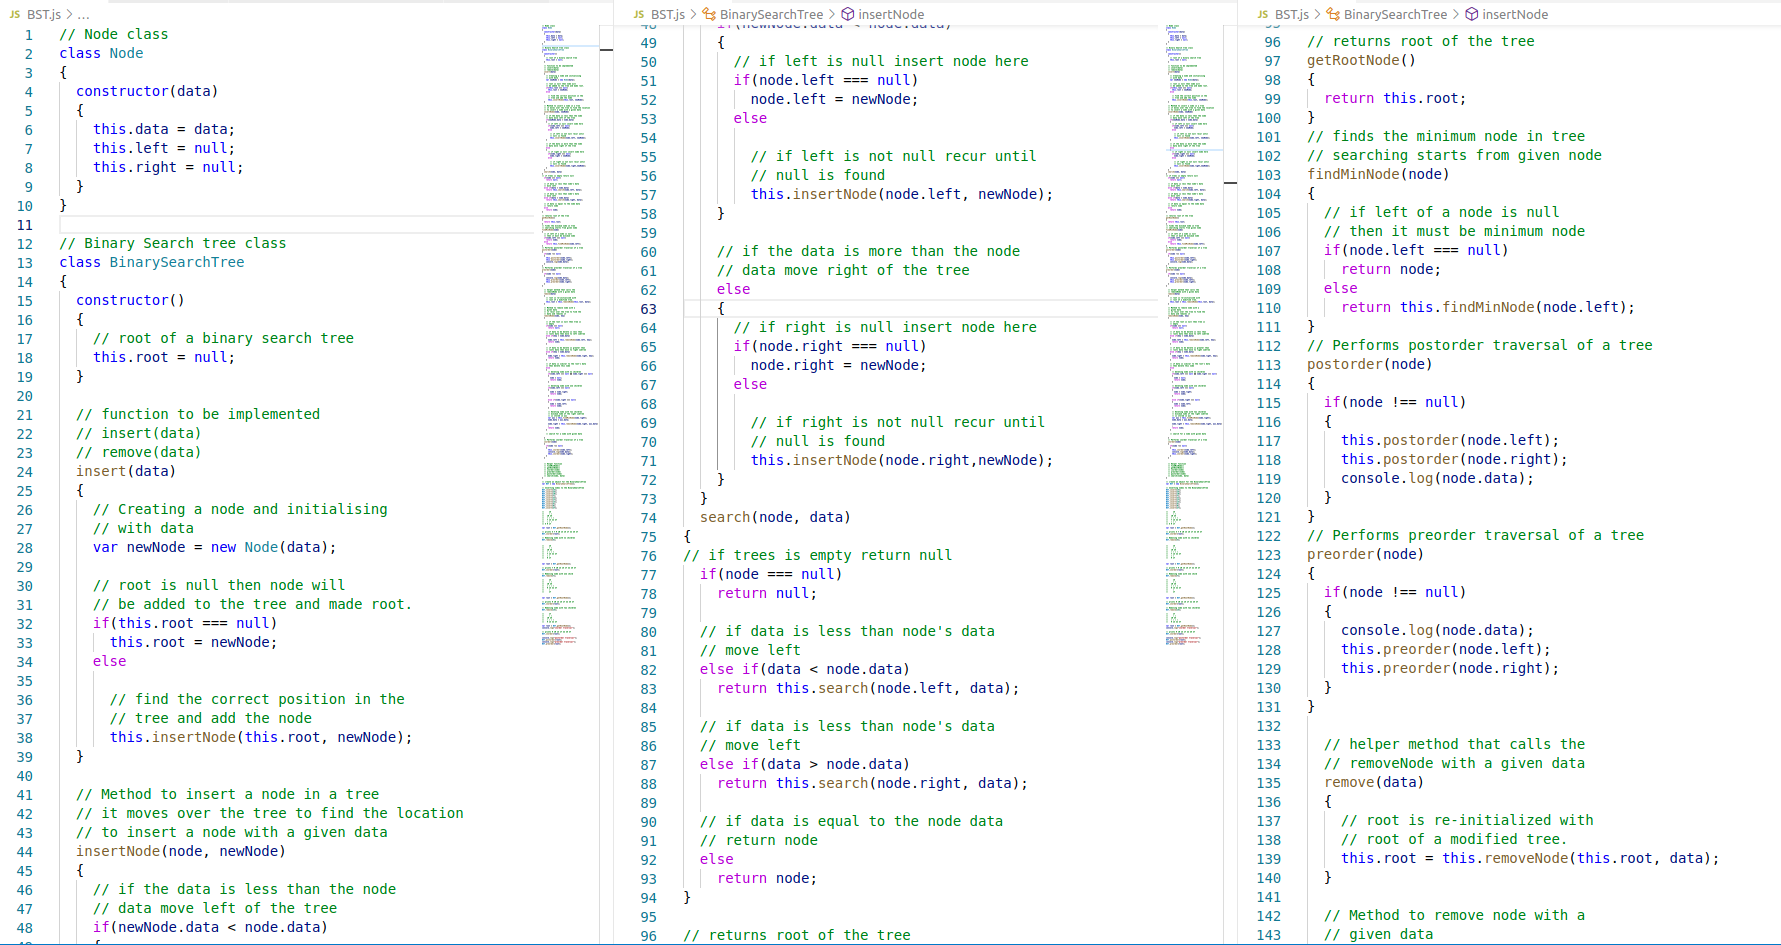
\includegraphics[width=1.1\linewidth]{Pictures/BST_Code1}
    	\caption{}
    	\label{fig:bstcode1}
    \end{figure}
    \begin{figure}[H]
    	\centering
    	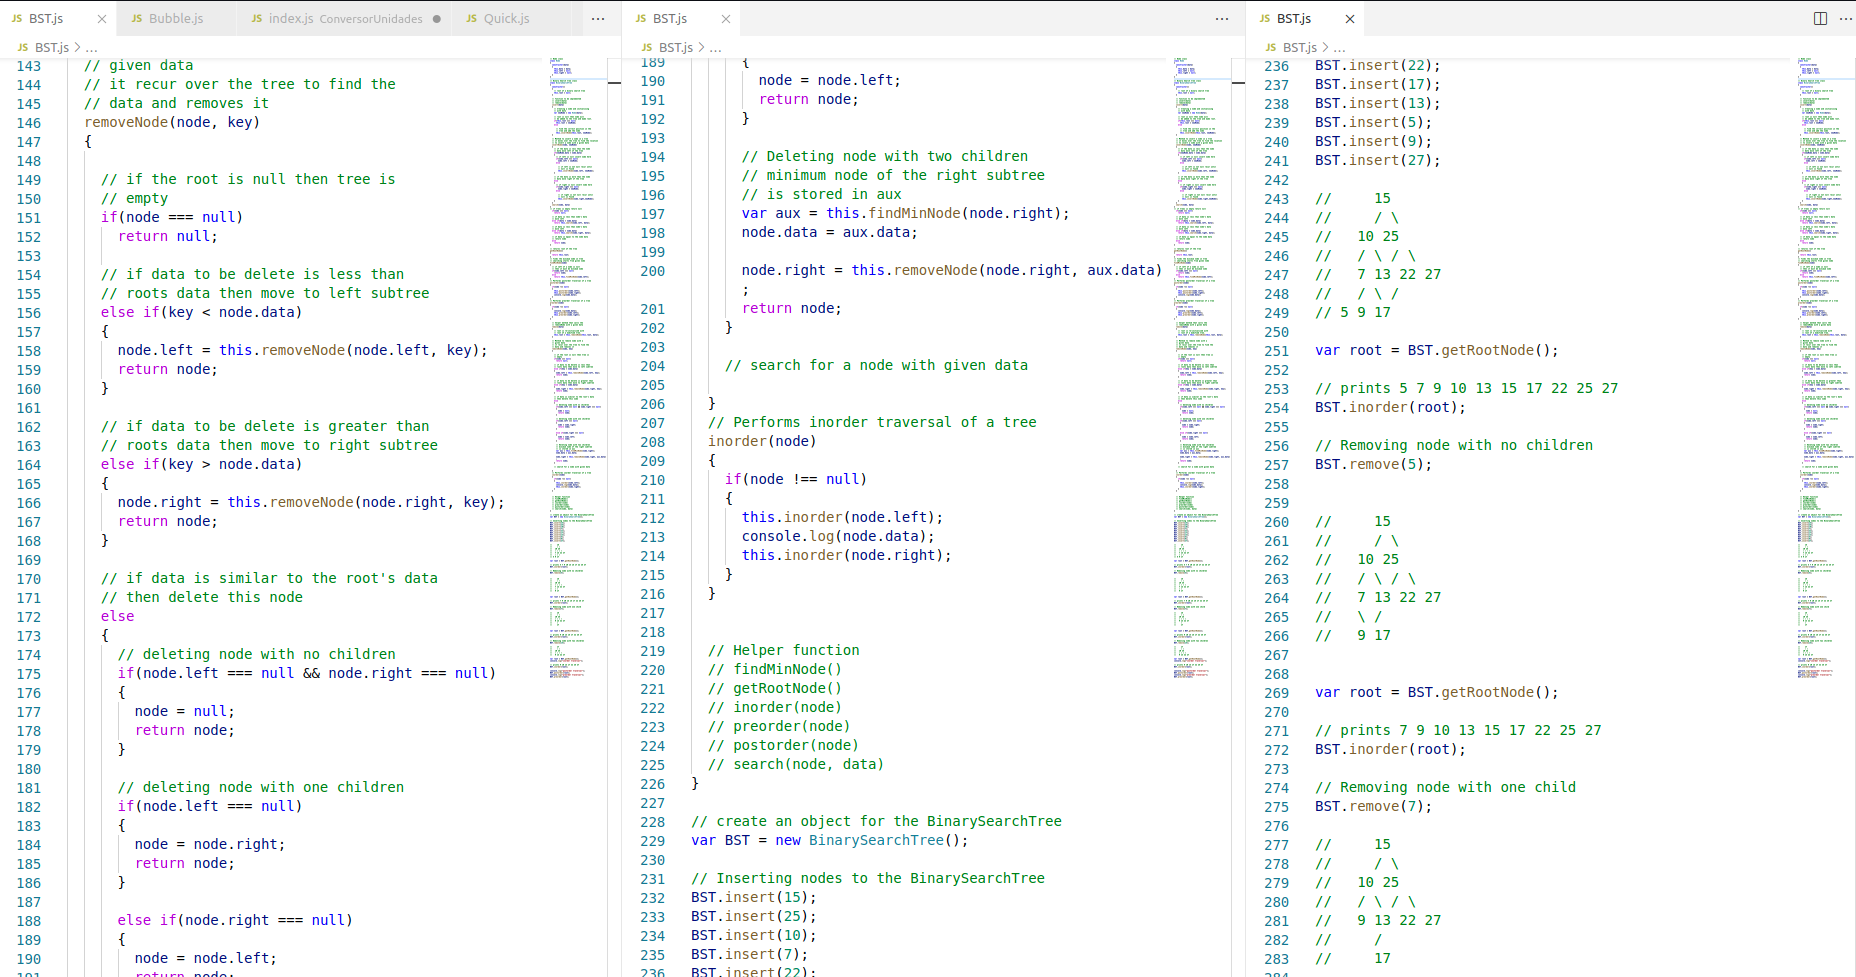
\includegraphics[width=1.1\linewidth]{Pictures/BST_Code2}
    	\caption{}
    	\label{fig:bstcode2}
    \end{figure}
    \begin{figure}[H]
    	\centering
    	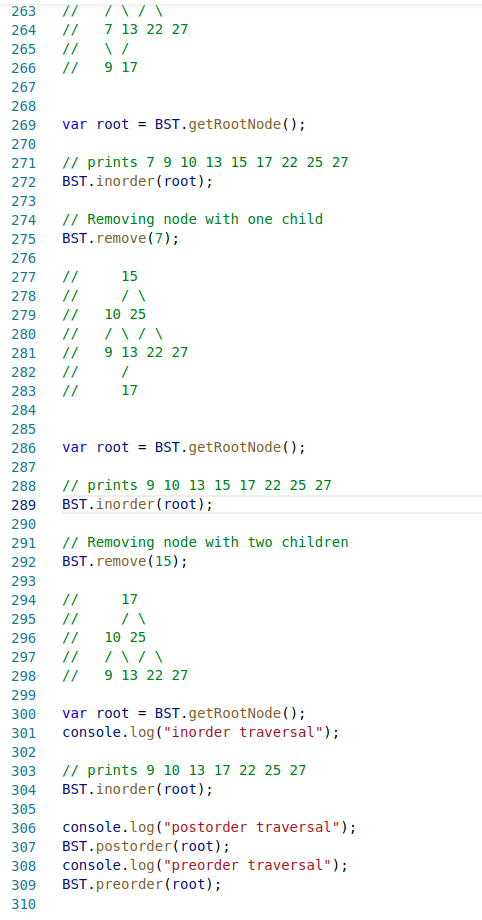
\includegraphics[width=0.9\linewidth]{Pictures/BST_Code3}
    	\caption{}
    	\label{fig:bstcode3}
    \end{figure}
    \begin{figure}[H]
    	\centering
    	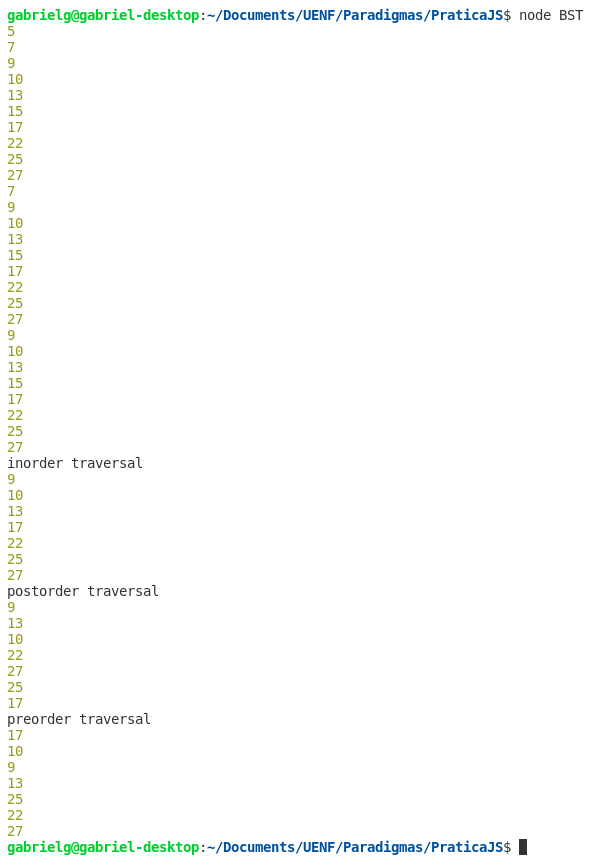
\includegraphics[width=0.9\linewidth]{Pictures/BST_Result}
    	\caption{}
    	\label{fig:bstresult}
    \end{figure}
    


    \section{Calculadora}
    O exemplo abaixo foi feito em JavaScript com HTML e CSS e interpretado pelo navegador.
    \begin{lstlisting}
    var valor1, valor2, operador;
    var readlineSync = require('readline-sync');
    operador = readlineSync.question("Qual operacao deseja efetuar (+) (-) (*) (/)? : \n");
    valor1 = parseFloat(readlineSync.question("Insira o primeiro numero: \n"));
    valor2 = parseFloat(readlineSync.question("Insira o segundo numero: \n"));
    
    function calcular(operator, value1, value2) {
    if (operator == "+") {
    return value1 + value2;
    } else if
    (operator == "-") {
    return value1 - value2;
    } else if
    (operator == "*") {
    return value1 * value2;
    } else if
    (operator == "/") {
    return value1 / value2;
    } else {
    throw new Error('Operacao invalida');
    }
    }
    
    
    console.log('O resultado e: ', calcular(operador, valor1, valor2))     
    \end{lstlisting}
    
    \subsection{Prints Calculadora}
	
	Imagens do código e do resultado, respectivamente: 
	\begin{figure}[H]
		\centering
		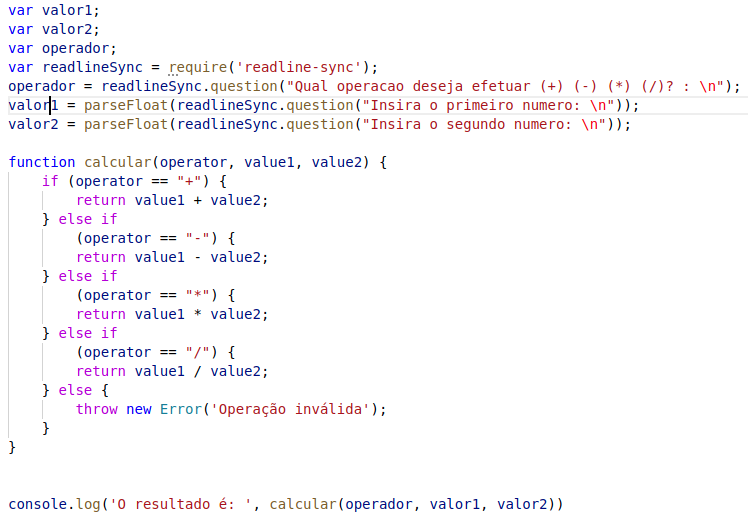
\includegraphics[width=0.9\linewidth]{Pictures/CalcCode}
		\caption{}
		\label{fig:calccode}
	\end{figure}
	\begin{figure}[H]
		\centering
		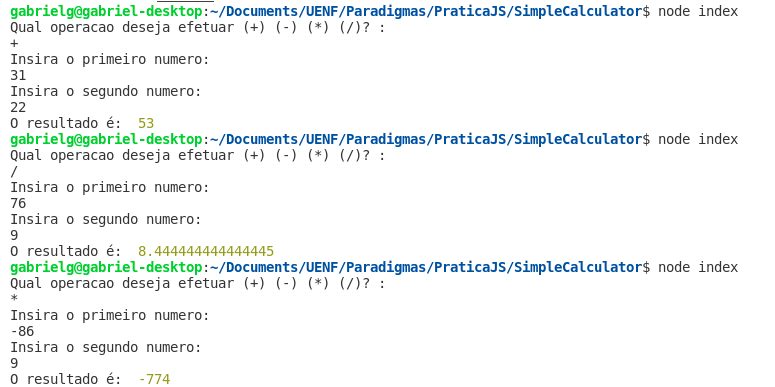
\includegraphics[width=0.9\linewidth]{Pictures/CalcResult}
		\caption{}
		\label{fig:calcresult}
	\end{figure}
	



    \section{Implementação do QuickSort}
	O algoritmo QuickSort é feito da seguinte forma no JavaScript:
	\newline
\begin{lstlisting}

// basic implementation, where pivot is the first element
function quickSortBasic(array) {
if(array.length < 2) {
return array;
}

var pivot = array[0];
var lesserArray = [];
var greaterArray = [];

for (var i = 1; i < array.length; i++) {
if ( array[i] > pivot ) {
greaterArray.push(array[i]);
} else {
lesserArray.push(array[i]);
}
}

return quickSortBasic(lesserArray).concat(pivot, quickSortBasic(greaterArray));
}

/******************* Testing Quick sort algorithm *********************/

// Returns a random integer between min (inclusive) and max (inclusive). Using Math.round() will give a non-uniform distribution, which we dont want in this case.

function getRandomInt(min, max) {
return Math.floor(Math.random() * (max - min + 1)) + min;
// By adding 1, I am making the maximum inclusive ( the minimum is inclusive anyway). Because, the Math.random() function returns a floating-point, pseudo-random number in the range from 0 inclusive up to but not including 1
}

var arr = [];

for (var i = 0; i < 10; i++) { //initialize a random integer unsorted array
arr.push(getRandomInt(1, 100));
}

console.log("Unsorted array: ");
console.log(arr); //printing unsorted array

arr = quickSortBasic(arr, 0, arr.length - 1);
console.log("Sorted array: ");
console.log(arr);


\end{lstlisting}
O código foi retirado de:
\url{https://javascript.plainenglish.io/quick-sort-algorithm-in-javascript-5cf5ab7d251b}


\subsection{Prints QuickSort}
	Código Fonte e imagem do resultado, respectivamente:
	\begin{figure}[H]
		\centering
		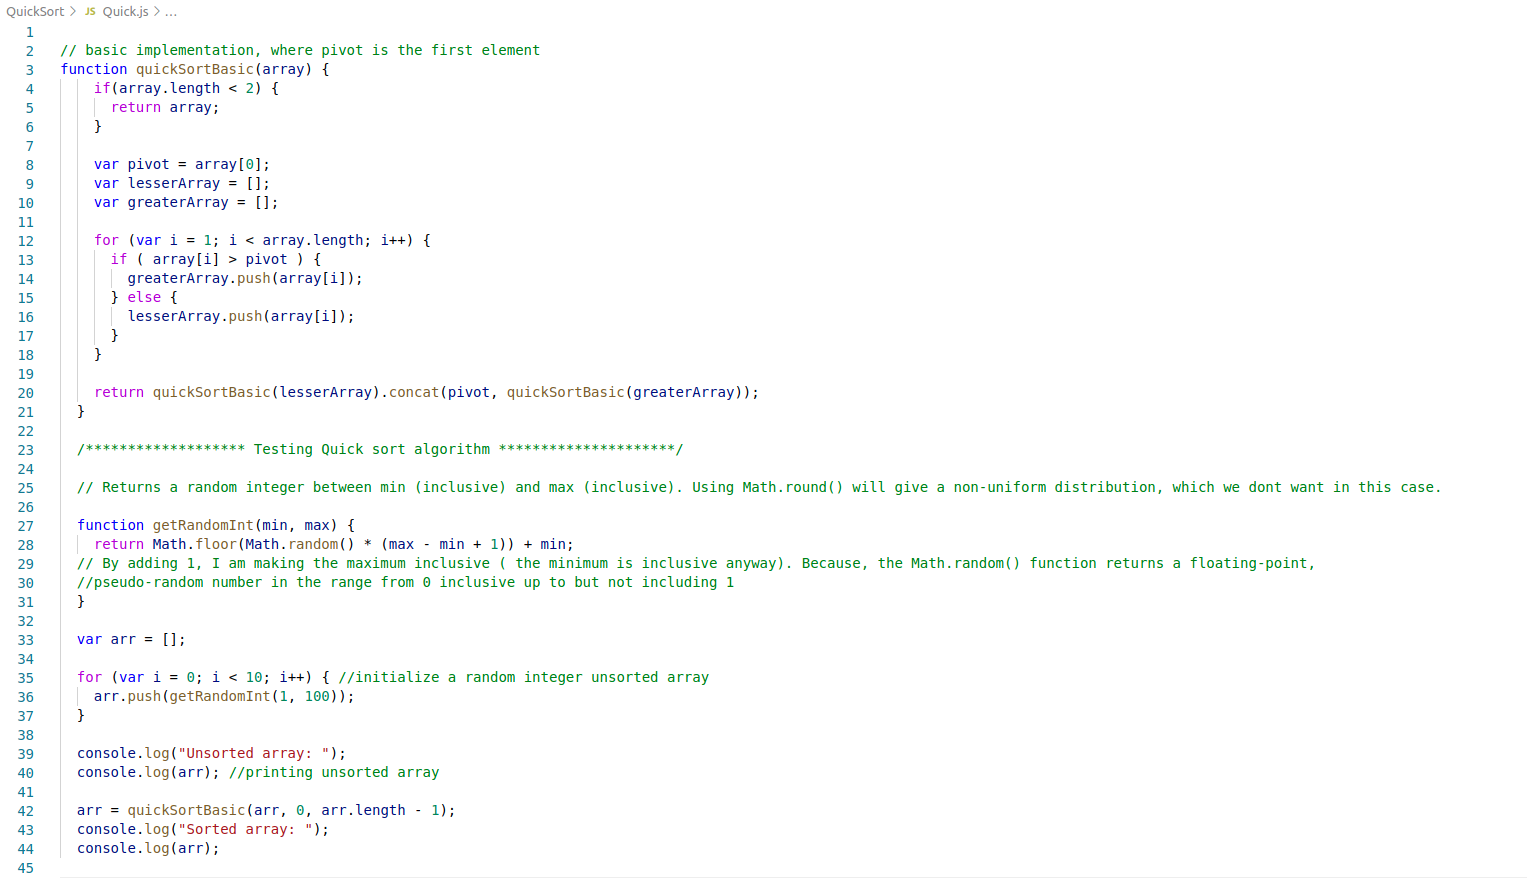
\includegraphics[width=0.95\linewidth]{Pictures/QuickCode}
		\caption{}
		\label{fig:quickcode}
	\end{figure}
	
	\begin{figure}[H]
		\centering
		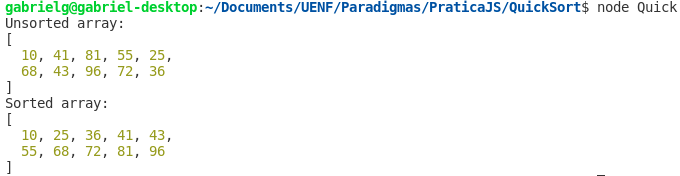
\includegraphics[width=0.95\linewidth]{Pictures/QuickResult}
		\caption{}
		\label{fig:quickresult}
	\end{figure}
	
	
	
 \section{Conversor de Temperatura}
 O código abaixo foi feito utilizando o módulo 'prompt-sync'.
 \begin{lstlisting}
 // TC/5 = (TF-32)/9 = (TK-273)/5
 
 const prompt = require('prompt-sync')();
 
 const temperatura = Number(prompt('Qual temperatura? '));
 
 
 const escala = prompt('Qual a escala da temperatura inserida? (1: Celsius; 2: Fahrenheit; 3: Kelvin)');
 
 switch(escala) {
 case '1':
 temperatura_fahrenheit = (temperatura/5)*9+32;
 temperatura_kelvin = (temperatura + 273.15);
 console.log("A temperatura: ", temperatura_kelvin, "K e ", temperatura_fahrenheit, "graus F");
 break;
 case '2':
 temperatura_celsius = ((temperatura-32)/9)*5;
 temperatura_kelvin = ((temperatura-32)/9)*5+273.15;
 console.log("A temperatura: ", temperatura_celsius, "graus C e ", temperatura_kelvin, "K");
 break;
 
 case '3':
 temperatura_fahrenheit = ((temperatura-273.15)/5)*9+32;
 temperatura_celsius = (temperatura)-273.15;
 console.log("A temperatura: ", temperatura_fahrenheit, "graus F e ", temperatura_celsius, "graus C")
 break;
 
 default:
 console.log('Insira uma escala valida de 1 a 3.');
 }
 \end{lstlisting}
 
 \subsection{Conversor de Temperatura Imagens}
 Código fonte e imagem do resultado:
\begin{figure}[h]
	\centering
	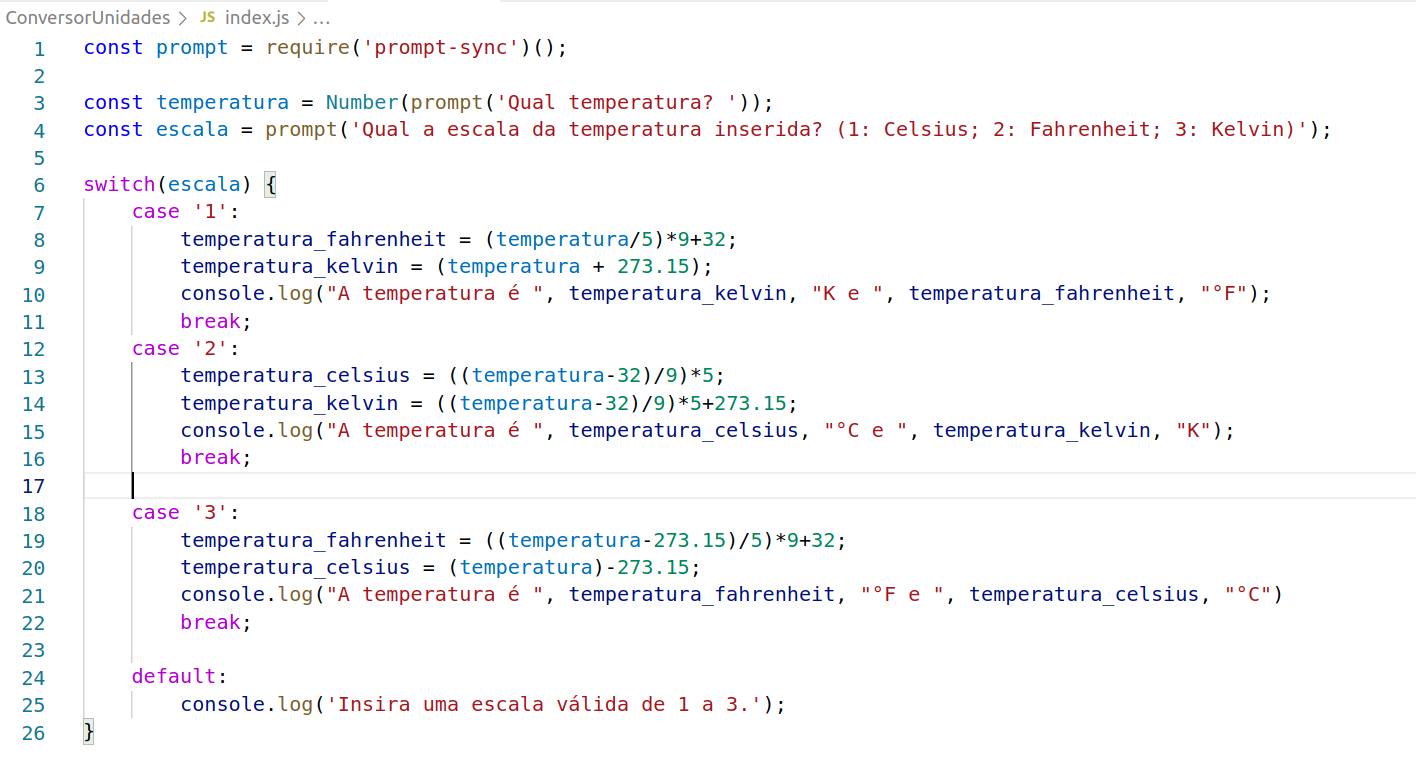
\includegraphics[width=1\linewidth]{Pictures/ConversorTempCode}
	\caption{}
	\label{fig:conversortempcode}
\end{figure}
\begin{figure}[h]
	\centering
	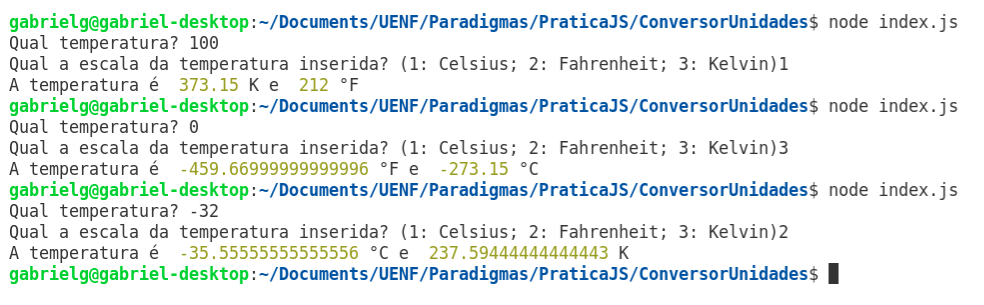
\includegraphics[width=0.9\linewidth]{Pictures/ConversorTempResultado}
	\caption{}
	\label{fig:conversortempresultado}
\end{figure}

	
	
	


	
% Prof. Dr. Ausberto S. Castro Vera
% UENF - CCT - LCMAT - Curso de Ci\^{e}ncia da Computa\c{c}\~{a}o
% Campos, RJ,  2021
% Disciplina: Paradigmas de Linguagens de Programa\c{c}\~{a}o


\chapter{Ferramentas existentes e utilizadas}

Neste cap\'{\i}tulo devem ser apresentadas pelo menos DUAS (e no m\'{a}ximo 5) ferramentas consultadas e utilizadas para realizar o trabalho, e usar nas aplica\c{c}\~{o}es. Considere em cada caso:
\begin{itemize}
  \item Nome da ferramenta (compilador-interpretador)
  \item Endere\c{c}o na Internet
  \item Vers\~{a}o atual e utilizada
  \item Descri\c{c}\~{a}o simples (m\'{a}x 2 par\'{a}grafos)
  \item Telas capturadas da ferramenta
  \item Outras informa\c{c}\~{o}es
\end{itemize}

    \section{Node JS}
    A linguagem JavaScript não está mais atrelada somente ao navegador. Por isso, para utilizar a linguagem sem precisar recorrer a um Browser, utiliza-se o nodeJS. O NodeJS, conhecido apenas como Node, nada mais é do que o V8 (Engine do JavaScript no navegador Google Chrome) fora do Chrome. Sendo assim, para instalar o Node basta entrar em https://nodejs.org e baixar a versão desejada. 
    
\begin{figure}[h]
	\centering
	
\includegraphics[width=0.3\linewidth]{Pictures/NodeLogo}
	\caption{}
	\label{fig:nodelogo}
\end{figure}
    
    \subsection{NVM}
    Devido a existência de várias versões do Node, o NVM - Node Version Manager - facilita o trabalho com versões diferentes. Por exemplo, se num projeto antigo decide-se pela versão 11.5, é possível com o NVM utilizar o node 11.5 sempre naquele projeto, mesmo após atualizar o node para versões mais recentes.


    \section{Visual Studio Code}
    Hoje em dia existem diversas versões de IDEs para as mais variadas linguagens de programação. Netbeans e Eclipse para o Java, Pycharm para o Python entre outras. IDEs feitas pensando especificamente em uma linguagem sempre tiveram vantagem em relação às IDEs multi-uso, como o sublime-text. Porém, com o Visual Studio Code, que chamarei de VSC, programar em várias linguagens é fácil e sem dor de cabeça. 
    O VSC é uma IDE fácil de usar, relativamente leve e permite a instalação de inúmeras extensões para tornar o desenvolvimento o mais produtivo possível.
    Portanto, para programar em JavaScript, o VSCode é uma das melhores IDEs disponíveis. É fácil programar para web utilizando JS, HTML e CSS, e além disso, vários recursos são disponibilizados pelo programa.
    
	\begin{figure}[h]
		\centering
		
\includegraphics[width=0.2\linewidth]{Pictures/VSC_Logo}
		\caption{}
		\label{fig:vsclogo}
	\end{figure}


    \section{Interpretador UVW}


    \section{Ambientes de Programa\c{c}\~{a}o IDE MNP} 
% Prof. Dr. Ausberto S. Castro Vera
% UENF - CCT - LCMAT - Curso de Ci\^{e}ncia da Computa\c{c}\~{a}o
% Campos, RJ,  2021
% Disciplina: Paradigmas de Linguagens de Programa\c{c}\~{a}o


\chapterimage{Conclusao.jpg} % Chapter heading image
\chapter{Conclus\~{o}es}


Os problemas enfrentados neste trabalho ...


O trabalho que foi desenvolvido em forma resumida ...

Aspectos n\~{a}o considerados que poderiam ser estudados ou \'{u}teis para ...



   \begin{figure}[H]
    \begin{center}
        \caption{Linguagens de programa\c{c}\~{a}o modernas} \label{ling2}
        
\includegraphics[width=12cm]{js3.png} \\
        {\tiny \sf Fonte: O autor }
    \end{center}
   \end{figure} 










\chapterimage{Bibliografia.png}
\bibliographystyle{alpha}
\bibliography{JavaScriptBib}
\addcontentsline{toc}{chapter}{\textcolor{ocre}{Bibliografia}}
%----------------------------------------------------------------------------------------
%	INDEX
%----------------------------------------------------------------------------------------

\cleardoublepage
\phantomsection
\setlength{\columnsep}{0.75cm}
\addcontentsline{toc}{chapter}{\textcolor{ocre}{Index}}
\printindex

%----------------------------------------------------------------------------------------
% Prof. Dr. Ausberto S. Castro Vera
% UENF - CCT - LCMAT - Curso de Ci\^{e}ncia da Computa\c{c}\~{a}o
% Campos, RJ,  2021
% Disciplina: Paradigmas de Linguagens de Programa\c{c}\~{a}o


\noindent
\textbf{Disciplina:} \textit{Paradigmas de Linguagens de Programa\c{c}\~{a}o \the\year}\\
\textbf{Linguagem:} \textit{Linguagem JavaScript}\\
\textbf{Aluno:} \textit{Gabriel Marques de Amaral Gravina}


\section*{Ficha de avalia\c{c}\~{a}o:}



\begin{tabular}{|p{12cm}|c|}
  \hline
  % after \\: \hline or \cline{col1-col2} \cline{col3-col4} ...
  \textbf{Aspectos de avalia\c{c}\~{a}o (requisitos m\'{\i}nimos)} & \textbf{Pontos} \\
  \hline
  Elementos b\'{a}sicos da linguagem (M\'{a}ximo: 01 pontos) &  \\
  $\bullet$ Sintaxe (vari\'{a}veis, constantes, comandos, opera\c{c}\~{o}es, etc.) &  \\
  $\bullet$ Usos e \'{a}reas de Aplica\c{c}\~{a}o da Linguagem &  \\
  \hline
  Cada elemento da linguagem (defini\c{c}\~{a}o) com exemplos (M\'{a}ximo: 02 pontos) &  \\
  $\bullet$ Exemplos com fonte diferenciada ( Courier , 10 pts, azul) & \\
  \hline
  M\'{\i}nimo 5 exemplos completos - Aplica\c{c}\~{o}es (M\'{a}ximo : 2 pontos) &  \\
  $\bullet$ Uso de rotinas-fun\c{c}\~{o}es-procedimentos, E/S formatadas &  \\
  $\bullet$ Menu de opera\c{c}\~{o}es, programas gr\'{a}ficos, matrizes, aplica\c{c}\~{o}es &  \\
  \hline
  Ferramentas (compiladores, interpretadores, etc.) (M\'{a}ximo : 2 pontos) &  \\
  $\bullet$ Ferramentas utilizadas nos exemplos: pelo menos DUAS&  \\
  $\bullet$ Descri\c{c}\~{a}o de Ferramentas existentes:  m\'{a}ximo 5&  \\
  $\bullet$ Mostrar as telas dos exemplos junto ao compilador-interpretador&  \\
  $\bullet$  Mostrar as telas dos resultados obtidos nas ferramentas &  \\
  $\bullet$ Descri\c{c}\~{a}o das ferramentas (autor, vers\~{a}o, homepage, tipo, etc.) &  \\
  \hline
  Organiza\c{c}\~{a}o do trabalho (M\'{a}ximo: 01 ponto) &  \\
  $\bullet$ Conte\'{u}do, Historia, Se\c{c}\~{o}es, gr\'{a}ficos, exemplos, conclus\~{o}es, bibliografia &  \\
  \hline
   Uso de Bibliografia (M\'{a}ximo: 01 ponto)&  \\
   $\bullet$ Livros: pelo menos 3&  \\
   $\bullet$ Artigos cient\'{\i}ficos: pelo menos 3 (IEEE Xplore, ACM Library)&  \\
   $\bullet$ Todas as Refer\^{e}ncias dentro do texto, tipo [ABC 04] & \\
   $\bullet$ Evite Refer\^{e}ncias da Internet & \\
   \hline
     &  \\
  Conceito do Professor (Opcional: 01 ponto) & \\
  \hline
   & \\
  \hfill Nota Final do trabalho: & \\
  \hline
\end{tabular}\\
\textit{Observa\c{c}\~{a}o:} Requisitos m\'{\i}nimos significa a \textit{metade} dos pontos


\end{document}

